%=======================================================================
%  Reionization_State_of_the_Art.tex
%
%  State of the art: the physics, observational constraints and driving
%  agents of the Epoch of Reionization (EoR).
%
%  Compiled from a curated corpus of 60 arXiv papers, downloaded into
%      ./Constraints/   (25 papers)  -- parameters of the EoR
%      ./Agents/        (35 papers)  -- drivers of ionization and heating
%
%  Build:  pdflatex -> bibtex -> pdflatex -> pdflatex
%  Bibliography: refs.bib (auto-generated from the arXiv API)
%=======================================================================
\documentclass[11pt,a4paper]{article}

\usepackage[margin=2.4cm]{geometry}
\usepackage[T1]{fontenc}
\usepackage[utf8]{inputenc}
\usepackage{amsmath,amssymb}
\usepackage{booktabs}
\usepackage{longtable}
\usepackage{array}
\usepackage{xcolor}
\usepackage[numbers,sort&compress]{natbib}
\usepackage[colorlinks=true,linkcolor=blue!55!black,citecolor=green!45!black,
            urlcolor=blue!55!black]{hyperref}
\usepackage{enumitem}
\usepackage{tabularx}
\usepackage{graphicx}
\graphicspath{{figures/}}
\newcommand{\srcfig}[1]{\par\smallskip\footnotesize\textit{Reproduced from #1.}}

\newcommand{\xHI}{\ensuremath{\langle x_{\rm HI}\rangle}}
\newcommand{\GHI}{\ensuremath{\langle \Gamma_{\rm HI}\rangle}}
\newcommand{\lmfp}{\ensuremath{\lambda_{\rm mfp}}}
\newcommand{\nion}{\ensuremath{\dot{n}_{\rm ion}}}
\newcommand{\xiion}{\ensuremath{\xi_{\rm ion}}}
\newcommand{\fesc}{\ensuremath{f_{\rm esc}}}
\newcommand{\Msun}{\ensuremath{{\rm M}_\odot}}
\newcommand{\cMpc}{\ensuremath{{\rm cMpc}}}
\newcommand{\pMpc}{\ensuremath{{\rm pMpc}}}
\newcommand{\Tzero}{\ensuremath{T_0}}
\newcommand{\flag}[1]{\textcolor{red}{\textsf{[#1]}}}
\newcommand{\tM}{\textsf{\scriptsize[M]}}
\newcommand{\tA}{\textsf{\scriptsize[A]}}
\newcommand{\tD}{\textsf{\scriptsize[D]}}
\newcommand{\pheader}[3]{%
  \medskip\par\noindent
  \colorbox{black!6}{\parbox{\dimexpr\textwidth-2\fboxsep}{%
    \textbf{#1}\; ---\; #2.\hfill \textit{corpus range:}\; #3}}\par\nobreak\smallskip}
\newenvironment{pbullets}
  {\begin{itemize}[nosep,leftmargin=1.6em,label=\textbullet]}
  {\end{itemize}\medskip}


\title{\bf The Epoch of Reionization: Observational State of the Art\\
       and a Catalogue of Ionizing and Heating Agents}
\author{Literature synthesis prepared for L.\ Carvalho}
\date{8 September 2026}

\begin{document}
\maketitle

\begin{abstract}
\noindent
This document summarises the current observational picture of the Epoch of
Reionization (EoR) and catalogues the candidate agents of hydrogen/helium
ionization and of intergalactic medium (IGM) heating, together with the
quantitative criteria the literature actually uses to decide whether a given
source population is \emph{dominant}, \emph{significant} or \emph{negligible}.
It is built from a corpus of 60 refereed/preprint papers selected for citation
impact and recency (1999--2026), stored as PDFs in the companion folders
\texttt{Constraints/} (25 papers) and \texttt{Agents/} (35 papers).
Every numerical value quoted below is traceable to a specific paper in that
corpus; nothing has been invented, and quantities that could not be sourced are
explicitly flagged.  Section~\ref{sec:flagged} lists the additional topics I
encountered but did \emph{not} include, pending your decision.
\end{abstract}

\tableofcontents
\listoffigures

%=======================================================================
\section{Scope, corpus and method}
\label{sec:method}
%=======================================================================

\subsection{How the corpus was assembled}

Candidate papers were surfaced by (i) programmatic queries to the arXiv API
(\texttt{astro-ph.CO}) across the source-physics and constraint-physics
sub-topics named in the task specification, and (ii) targeted retrieval of
landmark papers by arXiv identifier.  Every identifier was verified against
the arXiv API before download (title, author list and posting date returned by
the API are stored in \texttt{corpus\_metadata.json}).  All 60 PDFs downloaded
successfully; no entry in the bibliography is a paper I did not retrieve.

Papers were partitioned into the two requested folders by their \emph{primary}
scientific claim:
\begin{itemize}[nosep]
  \item \texttt{Constraints/} --- papers whose main result is a measurement of,
        or an inference on, a parameter that characterises the EoR
        ($\tau$, \xHI$(z)$, \GHI, \lmfp, \Tzero, $T_{\rm S}$, bubble size,
        $z_{\rm end}$, $z_{50}$).
  \item \texttt{Agents/} --- papers whose main result is the identification or
        quantification of the \emph{contribution} of a source population or a
        physical channel (LyC photons, X-rays, cosmic rays, Ly$\alpha$ photons,
        secondary electrons) to ionization and/or heating.
\end{itemize}
Several papers legitimately straddle the boundary (e.g.\ \citet{HERA2022}
simultaneously reports a power-spectrum upper limit and an $L_{\rm X}/{\rm SFR}$
constraint).  In those cases the folder assignment follows the paper's
\emph{stated} headline result; the full corpus table
(Appendix~\ref{app:corpus}) records the assignment explicitly.

\subsection{Provenance conventions used throughout}
\label{sec:provenance}

\begin{itemize}[nosep]
  \item Uncertainties are reproduced exactly as quoted by the source paper,
        together with the confidence level the source states (68\%, 95\%, 99\%,
        or ``$1\sigma$'').  Where a source gives no confidence level I say so.
  \item Citation counts are \emph{not} used as evidence for any physical claim.
        Where I mention them (Appendix~\ref{app:corpus}) they come from the
        Semantic~Scholar API, retrieved 8~September~2026, and are known to
        undercount astronomy literature relative to NASA~ADS; treat them as a
        relative ranking only.
  \item BibTeX keys are built from the \emph{arXiv posting year}, which for
        some entries differs from the journal year (e.g.\ \texttt{Atek2023} is
        Nature~2024; \texttt{HERA2022} is ApJ~2023).
  \item \flag{flagged} marks a statement I could not verify from the corpus.
  \item \textbf{Figures.}  Every figure in this document is the \emph{original
        published figure}, extracted directly from the PDF in
        \texttt{Agents/} or \texttt{Constraints/} at 300\,dpi with
        \texttt{pdftocairo}; none has been redrawn, recoloured or replotted.
        Each caption names the source paper and figure number.  They are
        reproduced here for private research use; any onward use requires the
        publisher's permission.  The extracted PNGs live in \texttt{figures/}.
\end{itemize}

\subsection{Source-consistency audit}
\label{sec:audit}

Every numerical value in this document has been checked against the text of the
PDF it cites, using the script \texttt{verify\_claims.py} (shipped alongside).
The procedure: 116 numeric claims were encoded as (citation key, required
numeric tokens); each paper PDF was converted to text with \texttt{pdftotext};
tokens were matched after Unicode/whitespace normalisation; and the surrounding
$\pm95$ characters of every match were read to confirm the number is used in the
sense claimed here, not merely present somewhere in the paper.

\paragraph{Result.}
114 of 116 claims verified on the first pass.  The audit found \textbf{two
substantive numerical errors}, both traceable to a single root cause, and both
now corrected:

\begin{enumerate}[nosep,leftmargin=1.6em]
  \item \textbf{\citet{Chaubal2026} (SPT-3G D1).}  The values originally quoted
        ($D^{\rm kSZ}_{3000}=1.75\pm0.86$, $D^{\rm tSZ}_{3000}=4.91\pm0.37\,
        \mu{\rm K}^2$, $\Delta^{50}z_{\rm re}<3.8$, $\Delta^{90}z_{\rm re}<6.1$)
        are the \emph{v1} values.  The PDF in \texttt{Constraints/} is v2, which
        reports $1.98\pm0.87$, $4.98\pm0.35\,\mu{\rm K}^2$,
        $\Delta^{50}z_{\rm re}<4.2$ and $\Delta^{90}z_{\rm re}<7.0$.
        Section~\ref{sec:ksz} now quotes v2.
  \item \textbf{\citet{Rosdahl2018} (SPHINX).}  The binary-star boost to
        $\fesc$ was quoted as $3.5\times$; the v2 PDF states ``about 3 times
        higher'', with a luminosity-weighted $8.5\%$ (binaries) versus $2.7\%$
        (singles), i.e.\ a factor $\approx3.1$.  Section~\ref{sec:agents} now
        quotes v2.
\end{enumerate}

\paragraph{Root cause.}
The arXiv API returns, for some entries, the abstract of an \emph{earlier}
version than the identifier it reports and than the PDF it serves.  Both errors
entered because a value was taken from an API abstract rather than from the
downloaded paper.  A systematic sweep comparing every API abstract against its
PDF flagged exactly two further cases: \citet{Chaubal2026} (the error above) and
\citet{Simmonds2024}, whose listing abstract says 15\,721 galaxies where the v2
PDF says 14\,652 --- a number this document never quoted, so no correction was
needed.  \textbf{Two provenance improvements} were also made: $h=0.6736$ is now
stated as derived from the published $H_0=(67.36\pm0.54)\,{\rm km\,s^{-1}
\,Mpc^{-1}}$ (the bare value $h$ does not appear in \citealt{Planck2018}), and
the \citet{Naidu2019} ``oligarch'' definition now carries its
$\log(M_\star/\Msun)>8$ condition, which had been dropped.

\paragraph{Limitation of the audit.}
Token matching cannot detect a number that is correct in the paper but attached
to the wrong claim here \emph{if} the same digits occur elsewhere in that paper.
The \citet{Rosdahl2018} error was of exactly this type and was caught only by
reading contexts by hand.  I read the matched context for all 116 claims, but
this is a manual step and I cannot certify it exhaustive.

\subsection{Independent numerical cross-checks performed}
\label{sec:crosscheck}

Two checks were run with \texttt{sympy}/Python (script:
\texttt{crosscheck\_reionization.py}, shipped alongside this file; all inputs
cited, no free parameters):

\begin{enumerate}[nosep]
  \item \textbf{Dimensional consistency} of the reionization ODE
        (Eq.~\ref{eq:qdot}) and of the recombination time (Eq.~\ref{eq:trec}):
        both pass under \texttt{sympy.physics.units.systems.si.dimsys\_SI}.
  \item \textbf{Order-of-magnitude closure of the photon budget.}  Using
        $\Omega_{\rm b}h^2=0.02237$, $Y_{\rm p}=0.2454$ and
        $H_0=(67.36\pm0.54)\,{\rm km\,s^{-1}\,Mpc^{-1}}$, i.e.\ $h=0.6736$
        \citep[][TT,TE,EE+lowE+lensing]{Planck2018}, the comoving mean hydrogen
        density is
        $\langle n_{\rm H}\rangle = 1.895\times10^{-7}\,{\rm cm^{-3}}
        = 5.566\times10^{66}\,\cMpc^{-3}$.  The measured ionizing emissivity
        $\nion \simeq 0.6\times10^{51}\,{\rm s^{-1}\,\cMpc^{-3}}$ at
        $4.9\le z\le6.0$ \citep{Gaikwad2023} therefore corresponds to
        $3.4$ ionizing photons per hydrogen atom per Gyr.  Independently,
        Eq.~\ref{eq:nion} with the fiducial $\fesc=0.2$,
        $\log_{10}\xiion=53.14\,[{\rm s^{-1}}/(\Msun\,{\rm yr^{-1}})]$
        of \citet{Robertson2015} and
        $\rho_{\rm SFR}\simeq0.01$--$0.02\,\Msun\,{\rm yr^{-1}\,\cMpc^{-3}}$
        gives $\nion=2.8$--$5.5\times10^{50}\,{\rm s^{-1}\,\cMpc^{-3}}$.
        The two routes agree to within a factor $\lesssim2$, which is the
        expected level given the $\fesc$ and $\rho_{\rm SFR}$ uncertainties.
\end{enumerate}

\noindent
\textbf{Not cross-checked:} every value quoted directly from a paper's abstract,
table or text (Sections~\ref{sec:observations}--\ref{sec:agents}) is reproduced
as published and has \emph{not} been re-derived here.  Where two papers in the
corpus disagree, the disagreement is reported rather than resolved
(Section~\ref{sec:tensions}).

%=======================================================================
\section{What observations establish about the EoR}
\label{sec:observations}
%=======================================================================

\subsection{The cosmological framework and the integral constraint}

Thomson scattering of CMB photons off free electrons produced by reionization
imprints an optical depth
\begin{equation}
  \tau = c\,\sigma_{\rm T}\int_0^{z_{\rm max}}
         \frac{n_{\rm e}(z)}{(1+z)\,H(z)}\,\mathrm{d}z ,
  \label{eq:tau}
\end{equation}
which is an \emph{integral} of the ionization history and therefore constrains
its total but not its shape.  The current values are
\begin{itemize}[nosep]
  \item $\tau = 0.054 \pm 0.007$ (68\% CL), from the final full-mission
        \emph{Planck} TT,TE,EE+lowE+lensing analysis \citep{Planck2018}.
  \item $\tau = 0.0566^{+0.0053}_{-0.0062}$ (68\% CL) from large-scale
        polarization alone, and $\tau = 0.059 \pm 0.006$ (68\% CL) in
        combination, using the improved SRoll2 HFI map-making
        \citep{Pagano2019}.  This corresponds to a mid-point reionization
        redshift $z_{\rm re} = 8.14 \pm 0.61$ (68\% CL) \emph{within a
        parametrised (tanh) reionization model} --- the model dependence of
        $z_{\rm re}$ is essential and is frequently under-stated.
  \item An independent, astrophysics-anchored route gives
        $\tau_{\rm reio} = 0.067 \pm 0.011$: \citet{MonteroCamacho2026} combine
        CMB \emph{excluding} large-scale polarization, BAO, quasar damping-wing
        \xHI\ measurements and dark-pixel limits within a Gompertzian
        reionization parametrisation, and find agreement with the
        polarization-based value.
\end{itemize}

\subsection{The end of reionization: $z_{\rm end}\simeq5.2$--$5.3$}
\label{sec:end}

Four independent Ly$\alpha$-forest diagnostics now converge on a
\emph{late} end to reionization.

\paragraph{Dark-pixel fraction (nearly model independent).}
Any pixel with detected transmission must be highly ionized; dark pixels may be
either.  The dark fraction is therefore an upper limit on \xHI\ requiring no
assumption about the ionizing background or the quasar continuum
\citep{McGreer2014}:
\begin{itemize}[nosep]
  \item $\xHI \le 0.06+0.05$ ($1\sigma$) at $z=5.9$ and
        $\xHI \le 0.04+0.05$ ($1\sigma$) at $z=5.6$, from 22 quasars
        \citep{McGreer2014};
  \item updated with 34 deep XQR-30 spectra using Ly$\beta$+Ly$\gamma$
        \citep{Davies2025}:
        $\xHI \le \{0.030+0.048,\;0.095+0.037,\;0.191+0.056,\;0.199+0.087\}$
        ($1\sigma$) at $\bar z=\{5.481,\,5.654,\,5.831,\,6.043\}$.
        The authors conclude that the bulk of reionization is finished by
        $z>6$, while a ``soft landing'' extending to $z\sim5.4$ remains allowed.
\end{itemize}

\paragraph{Opacity fluctuations.}
\citet{Becker2014} discovered a $\sim110\,h^{-1}\,$Mpc trough with
$\tau_{\rm eff}\gtrsim7$ extending to $z\simeq5.5$ towards ULAS~J0148+0600, and
showed that the sightline-to-sightline scatter at $z\simeq5.6$--$5.8$ requires
volume-weighted \xHI\ fluctuations a factor $\ge3$ larger than density
fluctuations alone can produce.  By $z\sim5$ the scatter is fully explained by
the density field.

\paragraph{Ly$\alpha$ transmission statistics.}
With 67 sightlines at $z>5.5$ (largely XQR-30), \citet{Bosman2021} find
homogeneous-UVB simulations consistent with the data at $z\le5.2$ ($<1\sigma$),
in mild tension at $z=5.3$ ($\sim2.5\sigma$), and \emph{ruled out} at $z\ge5.4$
($>3.5\sigma$).  Reionization-related fluctuations therefore persist to at
least $z=5.3$ ($t=1.1\,$Gyr).

\paragraph{Dark gaps.}
Using 55 quasars, \citet{Zhu2021} measure the fraction of sightlines with gaps
longer than $30\,h^{-1}\,$Mpc: $F_{30}\simeq0.9,\,0.6,\,0.15$ at
$z=6.0,\,5.8,\,5.6$, with nine ultra-long ($L>80\,h^{-1}\,$Mpc) gaps at $z<6$
and long gaps persisting to $z\simeq5.3$.

\medskip\noindent
Radiative-transfer modelling of the emissivity, mean free path and neutral
fraction jointly favours completion at $z\simeq5.2$ \citep{Gaikwad2023}.

\subsection{The mid-point and the neutral fraction at $z=6$--$10$}
\label{sec:midpoint}

\begin{longtable}{@{}l l l l@{}}
\caption{Volume-averaged neutral hydrogen fraction \xHI\ from the corpus.
Uncertainties and confidence intervals are exactly as quoted by the source.}
\label{tab:xhi}\\
\toprule
Redshift & \xHI & Probe & Reference \\
\midrule
\endfirsthead
\toprule
Redshift & \xHI & Probe & Reference \\
\midrule
\endhead
\bottomrule
\endfoot
$5.481$ & $\le 0.030+0.048$ ($1\sigma$) & Ly$\beta$/Ly$\gamma$ dark pixels & \citet{Davies2025} \\
$5.654$ & $\le 0.095+0.037$ ($1\sigma$) & Ly$\beta$/Ly$\gamma$ dark pixels & \citet{Davies2025} \\
$5.6$   & $\le 0.04+0.05$ ($1\sigma$)   & Ly$\alpha$/Ly$\beta$ dark pixels & \citet{McGreer2014} \\
$5.831$ & $\le 0.191+0.056$ ($1\sigma$) & Ly$\beta$/Ly$\gamma$ dark pixels & \citet{Davies2025} \\
$5.9$   & $\le 0.06+0.05$ ($1\sigma$)   & Ly$\alpha$/Ly$\beta$ dark pixels & \citet{McGreer2014} \\
$6.00$  & $0.174^{+0.093}_{-0.109}$     & Forward-modelled $\tau_{\rm eff}$ & \citet{Gaikwad2023} \\
$6.043$ & $\le 0.199+0.087$ ($1\sigma$) & Ly$\beta$/Ly$\gamma$ dark pixels & \citet{Davies2025} \\
$6.10$  & $0.21^{+0.17}_{-0.07}$ (ATON) & Quasar damping wing (stacked)     & \citet{Durovcikova2024} \\
$6.46$  & $0.21^{+0.33}_{-0.07}$ (ATON) & Quasar damping wing (stacked)     & \citet{Durovcikova2024} \\
$6.87$  & $0.37^{+0.17}_{-0.17}$ (ATON) & Quasar damping wing (stacked)     & \citet{Durovcikova2024} \\
$\sim7$ & $0.59^{+0.11}_{-0.15}$        & Ly$\alpha$ EW of LBGs (Bayesian)  & \citet{Mason2017} \\
$7.09$  & $0.48\pm0.26$ (68\% cred.)    & Damping wing, ULAS~J1120+0641     & \citet{Davies2018} \\
$7.12^{+0.06}_{-0.08}$ & $0.53^{+0.18}_{-0.47}$ & JWST galaxy damping wings & \citet{Umeda2023} \\
$7.54$  & $0.60^{+0.20}_{-0.23}$ (68\% cred.) & Damping wing, ULAS~J1342+0928 & \citet{Davies2018} \\
$9.91^{+1.49}_{-1.15}$ & $0.92^{+0.08}_{-0.10}$ & JWST galaxy damping wings & \citet{Umeda2023} \\
\end{longtable}

\noindent
Global inferences that combine these probes give:
\begin{itemize}[nosep]
  \item EoR mid-point in $6.9 < z < 7.6$, with large spatial fluctuations in the
        IGM ionization state \citep{Fan2022}.
  \item $z_{50} = 7.16^{+0.15}_{-0.12}$ and a duration $\Delta z_{\rm re} < 1.8$
        (95\% credibility) from a joint Bayesian analysis of \emph{Planck}+SPT
        CMB power spectra, Lyman-line \xHI\ data, and 21-cm upper limits from
        HERA, LOFAR and the MWA \citep{Sims2025}.  This is model dependent, as
        the authors stress.
  \item An observationally-derived ionizing budget from 1428 JWST/NIRSpec
        spectra yields an \xHI$(z)$ history ending at $z\sim5.8$
        \citep{Giovinazzo2026}.
\end{itemize}

\begin{figure}[htbp]
\centering
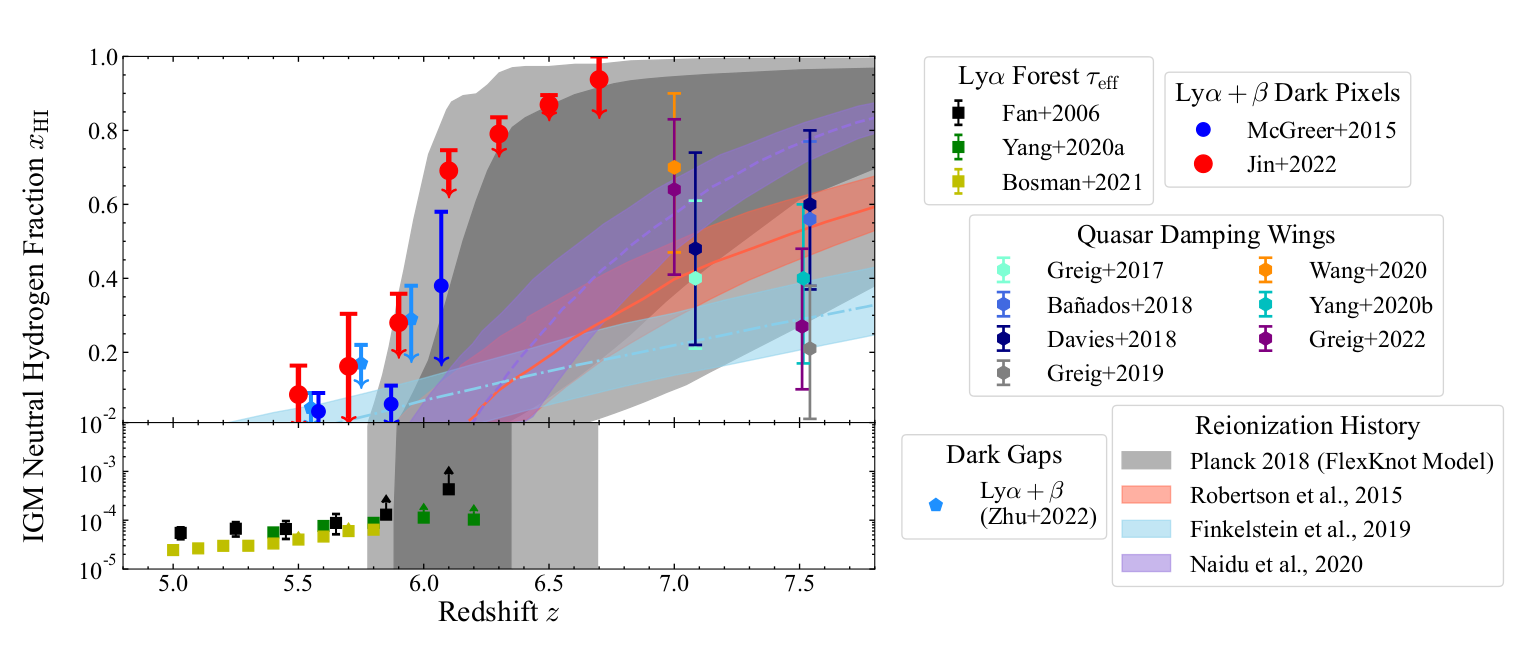
\includegraphics[width=\textwidth]{fig_reionization_history.png}
\caption[Reionization history]{\textbf{The reionization history as constrained by quasar
absorption.}  All data points are quasar-absorption constraints; the dark (light)
grey band is the $1\sigma$ ($2\sigma$) CMB constraint from \citet{Planck2018};
the red, blue and purple bands are the $1\sigma$ histories of the
\citet{Robertson2015}, \citet{Finkelstein2019} and \citet{Naidu2019} models
respectively.  Note the two-panel split: below $z\simeq6$ the forest measures
$x_{\rm HI}\sim10^{-5}$--$10^{-4}$ (lower panel, log scale), so the transition
spans four orders of magnitude in neutral fraction over $\Delta z\lesssim1$.
The model bands diverge most where the data are weakest, $z\gtrsim7$.
\srcfig{\citet{Fan2022}, Figure 16 (figure therein adapted from Jin et al.\ 2022)}}
\label{fig:history}
\end{figure}

\paragraph{Caveat on the damping-wing systematic.}
\citet{Durovcikova2024} report \xHI\ values that differ substantially depending
on which simulation grid is used to interpret the same stacked spectra: at
$\langle z\rangle=6.46$ they obtain $0.21^{+0.33}_{-0.07}$ with ATON but
$0.57^{+0.26}_{-0.47}$ with CROC.  The simulation suite is thus a leading
systematic, not a detail.  They simultaneously constrain the mean quasar
lifetime to $t_{\rm Q}\lesssim7\,$Myr in all bins.

\subsection{The ionizing background: \GHI, \lmfp\ and \nion}
\label{sec:uvb}

The three quantities are linked: in the local-source approximation the
photoionization rate scales as $\Gamma_{\rm HI}\propto \epsilon_\nu\,\lmfp$,
so a measurement of two determines the third.  Formally,
\begin{equation}
  \Gamma_{\rm HI} = \int_{\nu_{912}}^{\infty}
      \frac{4\pi J_\nu}{h\nu}\,\sigma_{\rm HI}(\nu)\,\mathrm{d}\nu .
  \label{eq:gamma}
\end{equation}
\flag{The proportionality prefactor relating $\Gamma_{\rm HI}$ to
$\epsilon_\nu\lmfp$ depends on the assumed spectral index and on the column
density distribution; I have not re-derived it, and none of the corpus papers
states it in closed form.}

\begin{table}[htbp]
\centering
\caption{Measured properties of the ionizing background from
\citet{Gaikwad2023}, Table~3 (XShooter+ESI quasar sample, forward-modelled
$\tau_{\rm eff}$ distribution).  $\Gamma_{12}\equiv\GHI/10^{-12}\,{\rm s^{-1}}$;
\lmfp\ in $h^{-1}\,\cMpc$; \nion\ in $10^{51}\,{\rm s^{-1}\,\cMpc^{-3}}$.
Uncertainties are total $1\sigma$ (modelling + cosmic variance + observational).
Compare the independent direct measurements of \citet{Becker2021}:
$\lmfp = 9.09^{+1.62}_{-1.28}\,\pMpc$ at $z=5.1$ and
$0.75^{+0.65}_{-0.45}\,\pMpc$ at $z=6.0$ (68\% confidence).}
\label{tab:uvb}
\begin{tabular}{@{}c c c c c@{}}
\toprule
$z$ & $\Gamma_{12}$ & \lmfp & $\langle f_{\rm HI}\rangle$ & \nion \\
\midrule
$4.90$ & $0.501^{+0.275}_{-0.232}$ & $50.1^{+33.1}_{-19.9}$ & $2.53^{+0.59}_{-0.44}\times10^{-5}$ & $0.600^{+0.304}_{-0.248}$ \\
$5.00$ & $0.557^{+0.376}_{-0.218}$ & $57.4^{+38.1}_{-21.1}$ & $2.27^{+0.84}_{-0.45}\times10^{-5}$ & $0.563^{+0.352}_{-0.207}$ \\
$5.20$ & $0.502^{+0.292}_{-0.193}$ & $40.8^{+22.3}_{-15.7}$ & $2.76^{+0.81}_{-0.56}\times10^{-5}$ & $0.668^{+0.461}_{-0.238}$ \\
$5.40$ & $0.372^{+0.217}_{-0.126}$ & $29.2^{+15.4}_{-10.2}$ & $3.53^{+15.08}_{-2.46}\times10^{-3}$ & $0.648^{+0.462}_{-0.225}$ \\
$5.60$ & $0.319^{+0.194}_{-0.120}$ & $23.0^{+11.7}_{-7.8}$  & $1.63^{+2.54}_{-0.83}\times10^{-2}$ & $0.666^{+0.402}_{-0.221}$ \\
$5.80$ & $0.178^{+0.194}_{-0.078}$ & $13.2^{+9.2}_{-5.8}$   & $9.36^{+6.18}_{-6.39}\times10^{-2}$ & $0.609^{+0.420}_{-0.141}$ \\
$6.00$ & $0.145^{+0.157}_{-0.087}$ & $8.32^{+7.53}_{-4.05}$ & $1.74^{+0.93}_{-1.09}\times10^{-1}$ & $0.701^{+0.357}_{-0.191}$ \\
\bottomrule
\end{tabular}
\end{table}

\begin{figure}[htbp]
\centering
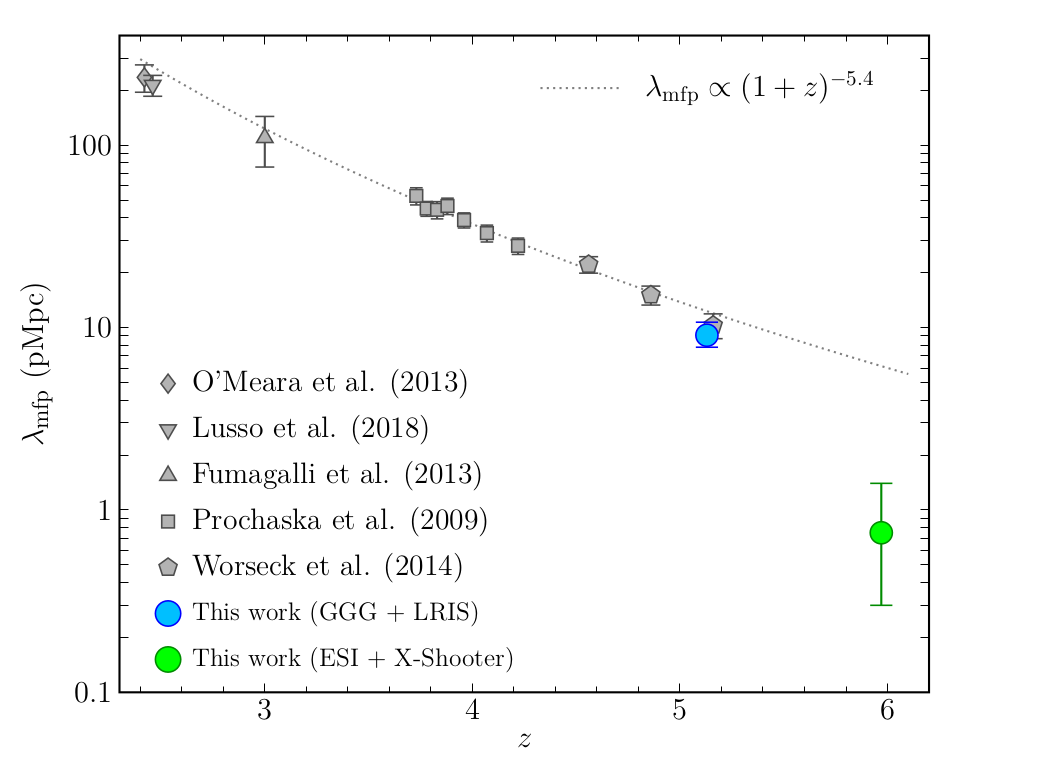
\includegraphics[width=0.62\textwidth]{fig_mean_free_path.png}
\caption[Mean free path of ionizing photons]{\textbf{The collapse of the mean
free path at $z=6$.}  Direct $\lmfp$ measurements against the
$\lmfp\propto(1+z)^{-5.4}$ power law fitted over $2.44<z<5.16$ by Worseck
et al.\ (2014).  The $z=5.1$ point (blue) sits on the extrapolation; the $z=6.0$
point (green) falls a factor $\sim7$ below it.  This is the single measurement
that most strongly forces reionization to end late.
\srcfig{\citet{Becker2021}, Figure 8}}
\label{fig:mfp}
\end{figure}

\begin{figure}[htbp]
\centering
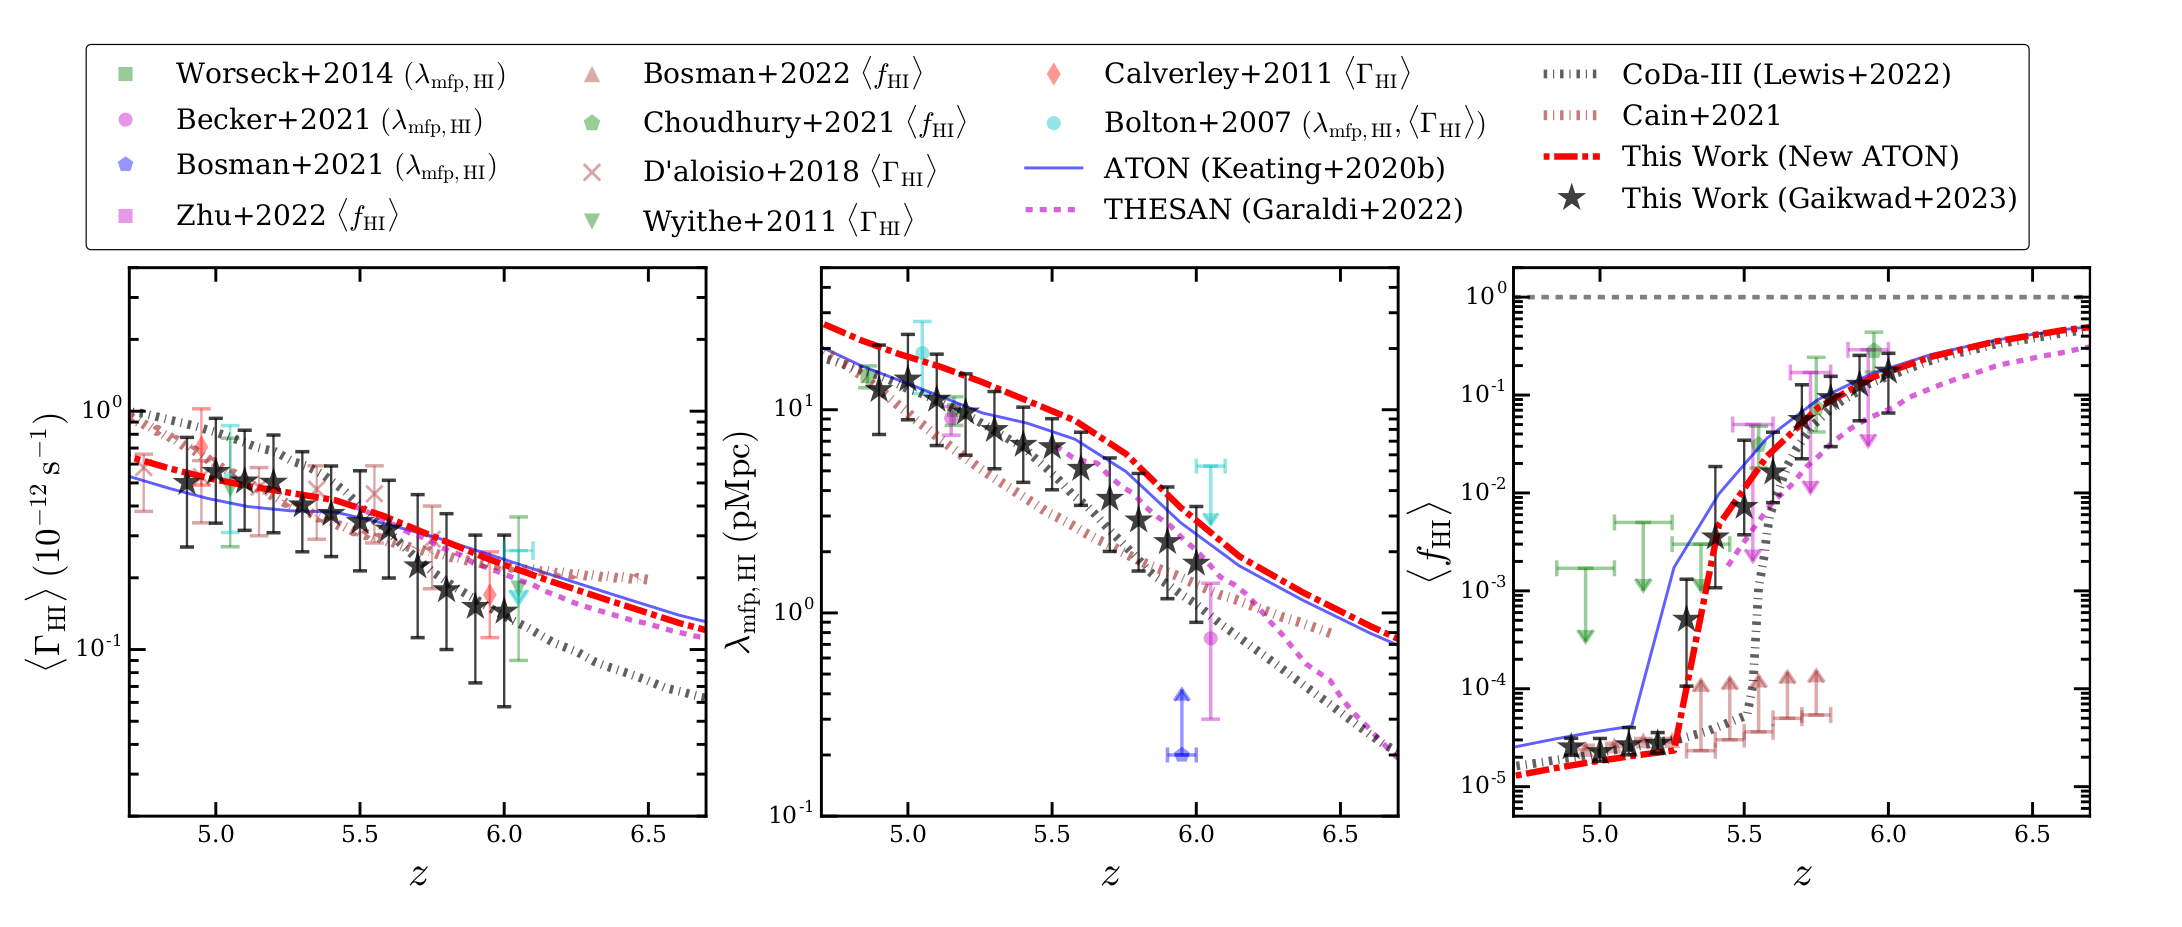
\includegraphics[width=\textwidth]{fig_uvb_evolution.png}
\caption[Ionizing background evolution]{\textbf{The three coupled quantities of
Table~\ref{tab:uvb}.}  Left to right: the photoionization rate $\GHI$, the mean
free path $\lmfp$, and the neutral fraction $\langle f_{\rm HI}\rangle$ over
$4.9\le z\le6.0$ (black stars), against literature measurements and the ATON,
THESAN, CoDa-III and Cain et al.\ simulations.  The near-vertical rise of
$\langle f_{\rm HI}\rangle$ between $z=5.2$ and $z=6.0$ --- four orders of
magnitude --- is the end of reionization; $\GHI$ falls by only a factor $\sim4$
across the same interval, because the drop is driven by $\lmfp$, not by the
sources.
\srcfig{\citet{Gaikwad2023}, Figure 10}}
\label{fig:uvb}
\end{figure}

Three physical statements follow directly from Table~\ref{tab:uvb}, which
Figure~\ref{fig:uvb} plots:
\begin{enumerate}[nosep]
  \item Between $z\sim5$ and $z\sim6$, \lmfp\ falls by a factor $\sim6$ and
        $\langle f_{\rm HI}\rangle$ rises by a factor $\sim10^4$
        \citep{Gaikwad2023}.  \citet{Becker2021} independently show the $z=6.0$
        mean free path lies well below extrapolations from lower redshift
        (Figure~\ref{fig:mfp}), and
        that neglecting the quasar proximity effect biases it high by a factor
        $\ge2$.
  \item The \emph{emissivity} \nion\ is, by contrast, nearly constant at
        $\simeq0.6\times10^{51}\,{\rm s^{-1}\,\cMpc^{-3}}$ across
        $4.9\le z\le6.0$.  The drop in \GHI\ is therefore driven by the
        collapsing mean free path, not by a collapsing source population.
  \item That emissivity corresponds to $3.4$ ionizing photons per hydrogen atom
        per Gyr (my cross-check, Section~\ref{sec:crosscheck}) --- i.e.\ the IGM
        at the end of the EoR is \emph{photon starved}: only a few photons per
        atom per Hubble time are available, so recombinations
        (Eq.~\ref{eq:trec}) matter at leading order.
\end{enumerate}

\subsection{The thermal state of the ionized IGM}
\label{sec:thermal}

The temperature at mean density, \Tzero, and the slope $\gamma$ of the
temperature--density relation $T=\Tzero\Delta^{\gamma-1}$ are measured from the
Ly$\alpha$ forest.  Note carefully: \emph{these measurements constrain the
already-ionized gas.}  The temperature of the residual \emph{neutral} IGM is
constrained only by 21-cm experiments (Section~\ref{sec:21cm}).

\begin{itemize}[nosep]
  \item From the width distribution of transmission spikes in five
        high-resolution $6<z\lesssim6.5$ quasar spectra compared to the Sherwood
        and Sherwood-Relics suites, \citet{Gaikwad2020} obtain
        $\Tzero = (11000\pm1600,\;10500\pm2100,\;12000\pm2200)\,$K at
        $z=(5.4,\,5.6,\,5.8)$, with $\gamma$ mildly steeper than isothermal.
        Spectral resolution $\le 8\,{\rm km\,s^{-1}}$ is required to resolve the
        spikes.
  \item A 400-simulation Cholla suite fit jointly to the H\,\textsc{i} 1D flux
        power spectrum in 14 bins over $2.2\le z\le5.0$ and to the
        He\,\textsc{ii} Ly$\alpha$ opacity in 5 bins over $2.4<z<2.9$ yields
        the two-peak thermal history of Figure~\ref{fig:thermal}
        \citep{Villasenor2021}: hydrogen
        reionization completing by $z\sim6.0$ with a first peak
        $\Tzero\sim1.3\times10^4\,$K, followed by He\,\textsc{ii} reionization
        completing by $z\sim3.0$ with a second peak
        $\Tzero\sim1.4\times10^4\,$K.
  \item Radiative-transfer simulations reach volume-averaged
        $\langle T\rangle\sim20{,}000\,$K at $z=6$ once the volume is
        essentially fully ionized ($\langle x_{\rm HII}\rangle=0.99998$)
        \citep{Eide2020}.
\end{itemize}

\begin{figure}[htbp]
\centering
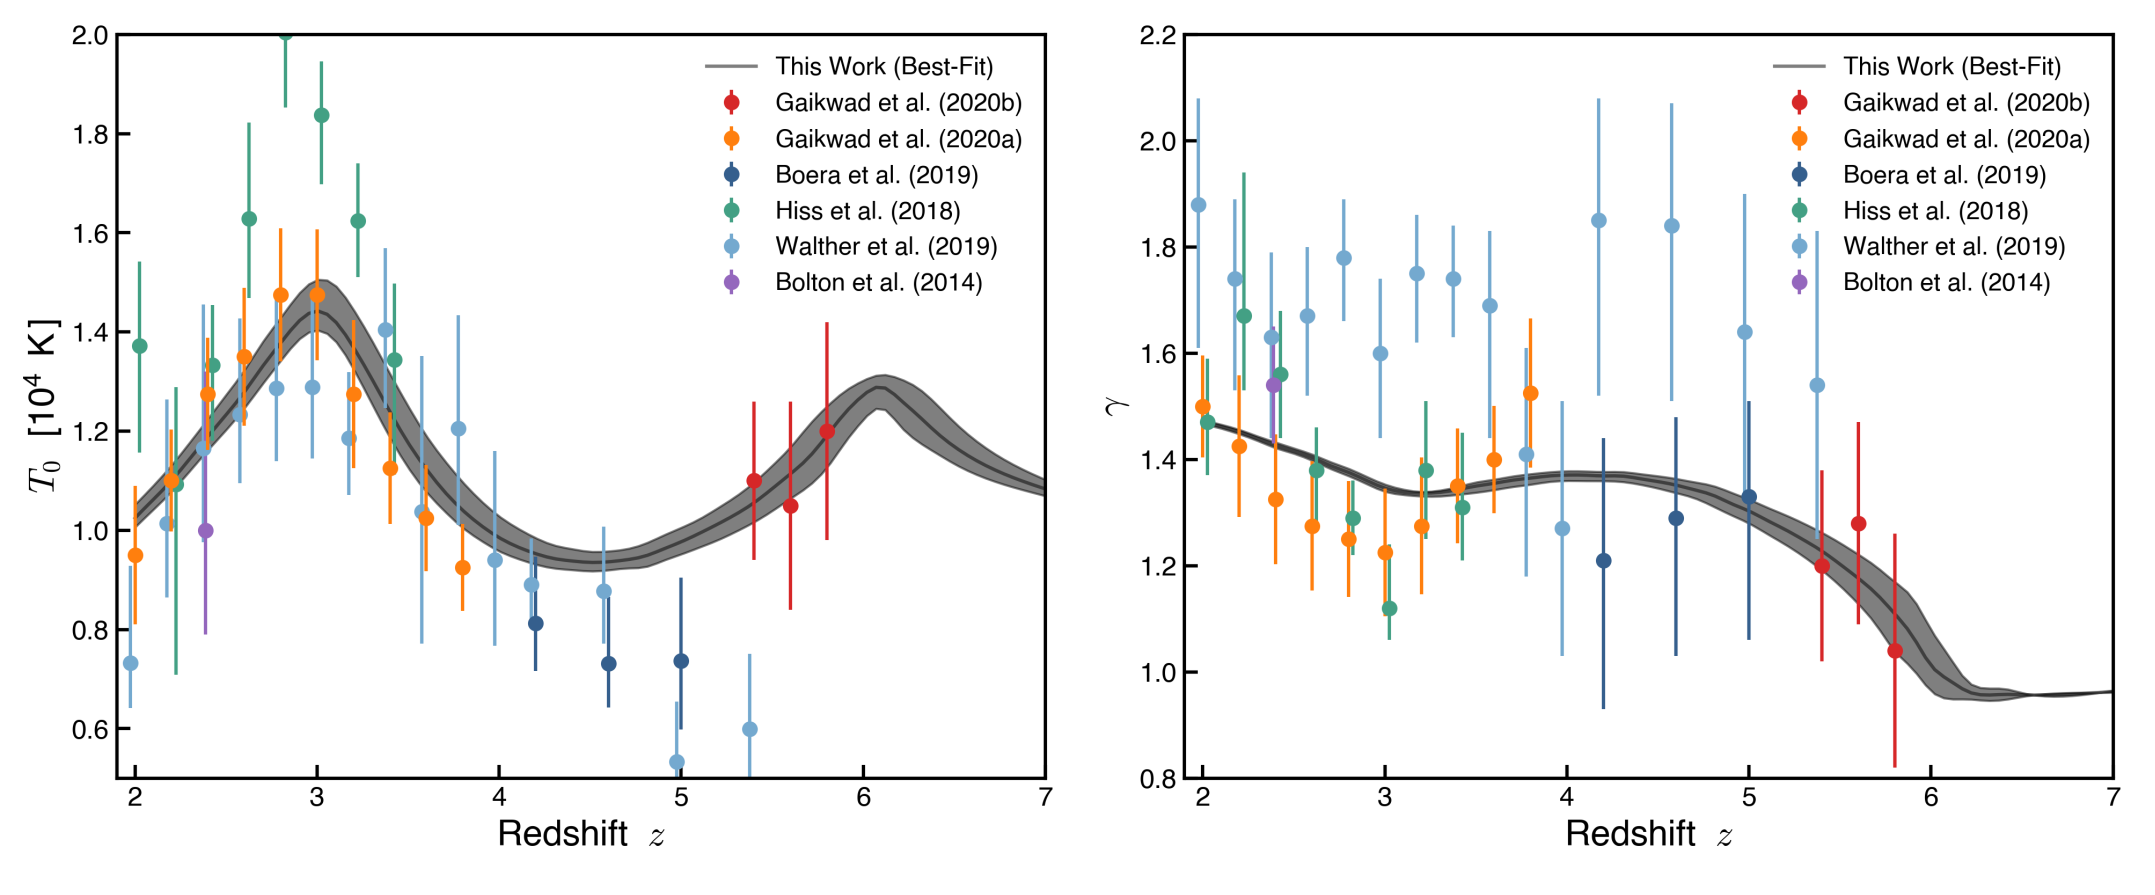
\includegraphics[width=\textwidth]{fig_thermal_history.png}
\caption[IGM thermal history]{\textbf{The two-peak thermal history of the
\emph{ionized} IGM.}  Redshift evolution of $\Tzero$ (left) and the
temperature--density slope $\gamma$ (right) from the best-fit model (black line,
95\% band) against Ly$\alpha$ forest measurements.  The peak at $z\simeq6$ is
hydrogen reionization; the peak at $z\simeq3$ is He\,\textsc{ii} reionization by
AGN.  These are the two heating events that stellar and AGN sources respectively
imprint on the IGM --- and note that nothing here constrains the \emph{neutral}
gas, which is the domain of Figure~\ref{fig:xray}.
\srcfig{\citet{Villasenor2021}, Figure 11}}
\label{fig:thermal}
\end{figure}

\subsection{21-cm constraints on the neutral, pre-reionization IGM}
\label{sec:21cm}

The 21-cm differential brightness temperature depends on the spin temperature
$T_{\rm S}$ through $\delta T_b\propto(1-T_{\rm CMB}/T_{\rm S})$, so upper
limits on the power spectrum translate into \emph{lower} limits on $T_{\rm S}$
and hence on the heating history.  No detection exists; all results below are
exclusions.

\paragraph{HERA Phase~I (94 nights) \citep{HERA2022}.}
\begin{itemize}[nosep]
  \item $\Delta^2(k=0.34\,h\,{\rm Mpc^{-1}}) \le 457\,{\rm mK^2}$ at $z=7.9$ and
        $\Delta^2(k=0.36\,h\,{\rm Mpc^{-1}}) \le 3496\,{\rm mK^2}$ at $z=10.4$
        (95\% confidence).
  \item Joint two-band fit: $T_{\rm S} > 11.0\,(35.2)\,$K at $z=7.9$ and
        $T_{\rm S} > 6.2\,(26.4)\,$K at $z=10.4$ at 95\% (68\%) credibility.
        Since $T_{\rm CMB}=24.3\,$K at $z=7.9$, ``cold reionization'' scenarios
        with enhanced power at $z=7.9$ are ruled out at $>95\%$ credibility.
  \item Corresponding intervals on the kinetic temperature:
        $3.2\,{\rm K} < T_{\rm K} < 313.2\,$K at $z=10.4$ and
        $13.0\,{\rm K} < T_{\rm K} < 4768\,$K at $z=7.9$.
  \item \textbf{Heating-source constraint:}
        $L_{\rm X<2\,keV}/{\rm SFR} \sim 10^{39.9}$--$10^{41.6}\,
        {\rm erg\,s^{-1}}\,(\Msun\,{\rm yr^{-1}})^{-1}$ (68\% HPD), tightening
        to $10^{40.4}$--$10^{41.8}$ at 95\%, under the prior
        $L_{\rm X<2\,keV}/{\rm SFR}<10^{42}$ (above which X-rays reionize the
        Universe too quickly).  More than 99\% of the posterior volume excludes
        the \emph{local}, metal-enriched $L_{\rm X}$--SFR relation continuing to
        high redshift; the data are consistent with low-metallicity HMXB models.
        This is the single most direct observational statement in the corpus
        about \emph{which} agent heated the IGM.
\end{itemize}

\begin{figure}[htbp]
\centering
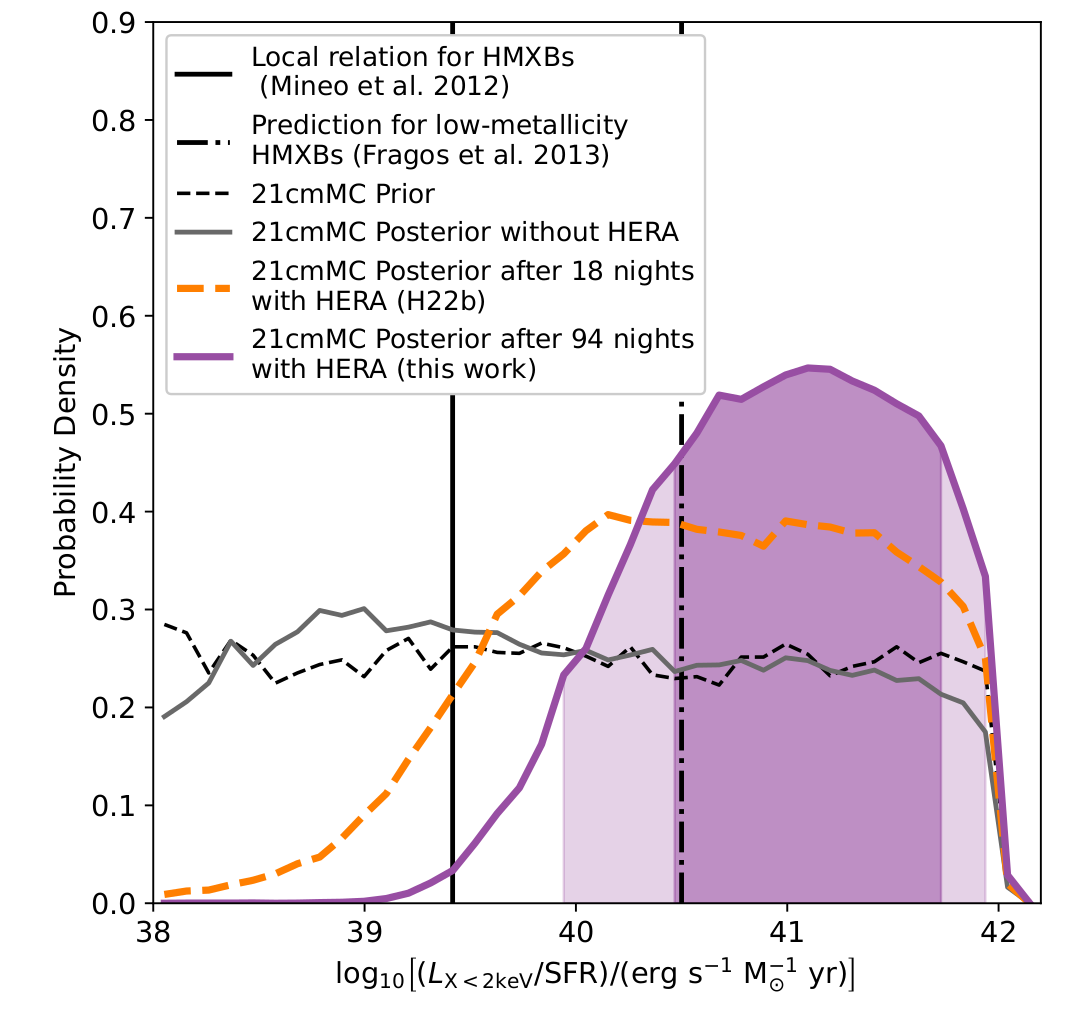
\includegraphics[width=0.66\textwidth]{fig_xray_heating.png}
\caption[X-ray heating efficiency from HERA]{\textbf{The strongest direct
observational statement about which agent heated the IGM.}  Marginalised
posterior on the soft X-ray luminosity per unit star formation,
$L_{\rm X<2\,keV}/{\rm SFR}$, with 68\% and 95\% credible intervals shaded.  The
solid vertical line is the \emph{local}, metal-enriched HMXB relation (Mineo
et al.\ 2012); the dash-dotted line is the prediction for low-metallicity HMXBs
(Fragos et al.\ 2013).  More than 99\% of the posterior volume lies above the
local relation, so the first galaxies cannot have followed it --- the data
require low-metallicity X-ray binaries.
\srcfig{\citet{HERA2022}, Figure 28}}
\label{fig:xray}
\end{figure}

\paragraph{LOFAR (10 nights) \citep{Ghara2025}.}
Interpreting the LOFAR upper limits with the \textsc{grizzly} code, models
disfavoured at $z=9.1$ correspond to an averaged ionized-plus-heated fraction
below $0.46$ ($\lesssim0.05$ at 68\%), an average gas temperature below $44\,$K
($4\,$K at 68\%), and a characteristic heated-region size
$\lesssim14\,h^{-1}\,$Mpc ($\lesssim3\,h^{-1}\,$Mpc at 68\%), at 95\% (68\%)
credibility.  The authors emphasise these are \emph{extreme} models driven by
rare large ionized/heated regions, and that the 68\% interval prefers an excess
radio background $>100\%$ of the CMB at $1.42\,$GHz while the 95\% interval
spans the whole prior --- i.e.\ the excess-radio-background degeneracy is not
broken.

\subsection{The 21-cm forest: a direct probe of the \emph{neutral} IGM temperature}
\label{sec:forest}

Absorption by intervening neutral hydrogen in the spectrum of a high-$z$
radio-loud source produces a ``21-cm forest''.  Because the optical depth scales
roughly as $\tau_{21}\propto x_{\rm HI}/T_{\rm S}$, the forest constrains the
temperature of exactly the phase that the Ly$\alpha$ forest cannot reach
(Section~\ref{sec:thermal}).

\begin{itemize}[nosep]
  \item \citet{Shao2023} show that the \emph{one-dimensional power spectrum} of
        the 21-cm forest breaks the otherwise severe degeneracy between warm
        dark matter (which suppresses small-scale structure) and early heating
        (which suppresses the absorption directly), allowing the SKA to
        constrain the dark matter particle mass and the heating level
        simultaneously.
  \item The first observationally informative result is now in hand.  Analysing
        archival uGMRT observations of J352$-$15 --- the brightest known
        radio-loud quasar in the EoR ($z=5.82$) --- at a sensitivity of
        $3.62\,{\rm mJy\,beam^{-1}}$ per $6.1\,$kHz channel,
        \citet{Soltinsky2026} obtain a null detection that nevertheless
        jointly constrains \xHI\ and the mean neutral-IGM temperature
        $\langle T_{\rm HI}\rangle$: at 68\% credibility, models with
        $\langle T_{\rm HI}\rangle \lesssim 27\,$K for $\xHI = 0.1$ at
        $z\approx5.6$ are disfavoured.  This independently indicates substantial
        pre-heating of the neutral IGM above the adiabatic cooling floor, in the
        same direction as the HERA $T_{\rm S}$ limits (Section~\ref{sec:21cm})
        but at much lower redshift and through a completely different
        systematic chain.
\end{itemize}

\subsection{The duration of reionization from the kinetic Sunyaev--Zel'dovich effect}
\label{sec:ksz}

Free electrons in bulk motion during a \emph{patchy} reionization Doppler-shift
CMB photons, producing an excess of small-scale temperature anisotropy.  Unlike
$\tau$, which is an integral of $n_{\rm e}(z)$ (Eq.~\ref{eq:tau}), the patchy
kSZ power at $\ell\simeq3000$ scales with the \emph{duration} of the transition,
and is therefore the only probe in this corpus that constrains $\Delta z_{\rm re}$
without assuming a source model.

\begin{itemize}[nosep]
  \item SPT-SZ + SPTpol report the first $\ge3\sigma$ measurement of kSZ power,
        $D^{\rm kSZ}_{3000} = 3.0 \pm 1.0\,\mu{\rm K}^2$, and, combined with
        their tSZ bispectrum, infer
        $\Delta z_{\rm re} = 1.0^{+1.6}_{-0.7}$
        ($\Delta z_{\rm re} < 4.1$ at 95\% confidence) \citep{Reichardt2020}.
  \item SPT-3G D1 measures
        $D^{\rm kSZ}_{3000} = 1.98 \pm 0.87\,\mu{\rm K}^2$ and
        $D^{\rm tSZ}_{3000} = 4.98 \pm 0.35\,\mu{\rm K}^2$ at $143\,$GHz (with the
        angular dependences of the SZ and CIB spectra free), and derives a 95\%
        limit on the duration between ionized fractions of 25\% and 75\% of
        $\Delta^{50} z_{\rm re} < 4.2$ (semi-analytic model), or between 5\% and
        95\% of $\Delta^{90} z_{\rm re} < 7.0$ (AMBER simulations)
        \citep{Chaubal2026}.
\end{itemize}

\noindent
\textbf{Caveat, stated by the authors themselves:} the inferred kSZ power depends
on the modelling of the tSZ--CIB correlation and on the assumed angular
dependence of the SZ spectra, and the reionization inference depends further on
the assumed level of homogeneous (late-time) kSZ power \citep{Chaubal2026}.
These limits are nevertheless consistent with, and independent of, the
$\Delta z_{\rm re} < 1.8$ (95\% credibility) obtained by \citet{Sims2025} from
the 21-cm/Lyman-line/CMB joint fit --- a genuine cross-check between two
unrelated data sets.

\subsection{Topology: reionization is patchy and inside-out}

\begin{itemize}[nosep]
  \item Excess Ly$\alpha$ opacity scatter beyond density fluctuations
        \citep{Becker2014,Bosman2021} and ultra-long dark gaps
        \citep{Zhu2021} require large-scale fluctuations in \lmfp, in the UV
        background, and/or in \xHI.
  \item JWST damping-wing analyses give ionized bubble radii evolving from
        $\log(R_{\rm b}/\cMpc)=1.67^{+0.14}_{-0.16}$ at $z\simeq7.1$ to
        $-0.69^{+0.89}_{-0.24}$ at $z\simeq9.9$ \citep{Umeda2023}.  These are
        up to a few dex larger than the cosmic average expected analytically at
        the same \xHI, but are comparable to merged bubbles around bright
        galaxies in simulations --- a selection effect that must be corrected
        before quoting a global \xHI.
  \item Different reionization source models produce distinct bubble size
        distributions and hence distinct large-scale slopes of the 21-cm power
        spectrum, which is the primary route by which upcoming 21-cm data will
        identify the dominant agent \citep{Kannan2021}.
\end{itemize}

\begin{figure}[htbp]
\centering
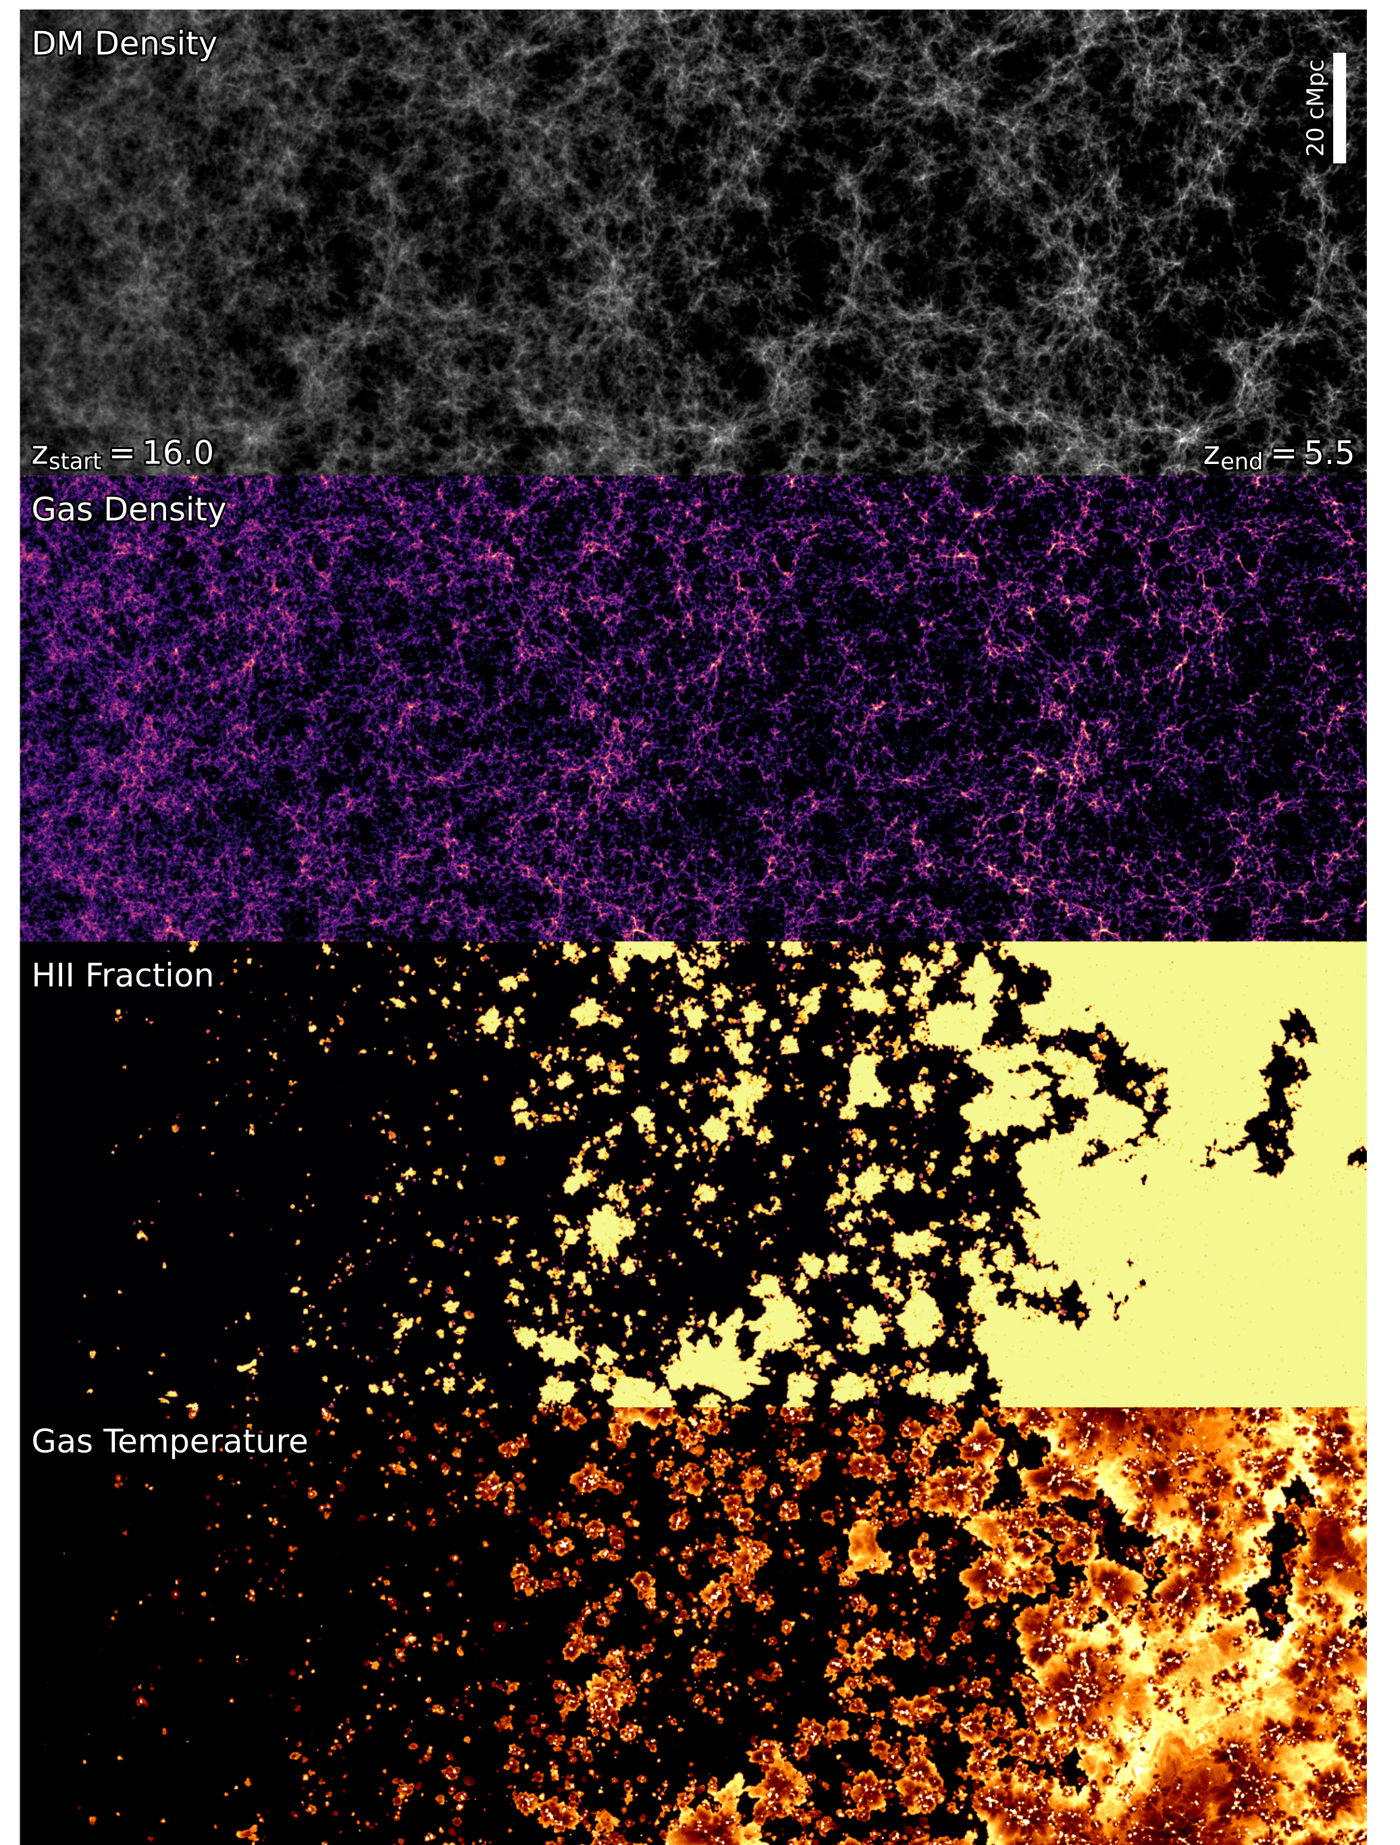
\includegraphics[width=0.80\textwidth]{fig_thesan_lightcone.png}
\caption[Reionization topology from simulation]{\textbf{Reionization is patchy
and inside-out.}  Mock light cones through the THESAN simulation from
$z_{\rm start}=16.0$ (left) to $z_{\rm end}=5.5$ (right), showing dark matter
density, gas density, H\,\textsc{ii} fraction and gas temperature.  The ionized
regions (third panel) nucleate around the densest structures, grow, and merge:
this is the geometry behind the opacity fluctuations of
Section~\ref{sec:end}, the bubble-size measurements of \citet{Umeda2023}, and
the selection bias that makes bubbles around bright galaxies unrepresentative.
The bottom panel shows that photoheating tracks ionization exactly, which is why
$\Tzero$ measures the ionized phase only.
\srcfig{\citet{Kannan2021}, Figure 2}}
\label{fig:thesan}
\end{figure}

\subsection{Helium reionization (a separate, later event)}

He\,\textsc{ii} requires $\ge54.4\,$eV photons.  Helium reionization is an
AGN-driven event, distinct from and much later than hydrogen reionization ---
but the usual shortcut for \emph{why} (``stars do not make such photons'') is
too strong, and is contradicted by evidence in this corpus.  The correct
statement is that stars do not supply \emph{enough} of them, and cannot supply
them where they are needed:
\begin{itemize}[nosep]
  \item Metal-free stars make a non-negligible number.  \citet{Murphy2021},
        Table~4, give $N_{\rm HeII}/N_{\rm H}=1.8\times10^{-2}$ for a top-heavy
        Pop~III IMF and $9.6\times10^{-3}$ for a Salpeter slope --- one to two
        per cent, not zero.  Rotating Pop~III models reaching
        $T_{\rm eff}\sim2\times10^{5}\,$K harden this further
        \citep{Wasserman2025}.
  \item It is observed.  Strong He\,\textsc{ii}\,$\lambda1640$ emission ---
        which requires He\,\textsc{ii} recombination and hence $>54.4\,$eV
        photons absorbed locally --- is detected at ${\rm EW}=21\pm4$\,\AA{} in
        a sub-$L_\star$ galaxy at $z=8.16$ \citep{Wang2022}, and at
        ${\rm EW}>20$\,\AA{} with \emph{no metal lines} at $z=10.6$ near GN-z11,
        where \citet{Maiolino2026} argue Pop~III stars are the only plausible
        explanation.
  \item The simulation most often cited for the strong claim assumes it away.
        \citet{Eide2020} conclude black holes ``are the only sources which can
        fully ionize helium'', but state that they ``do not account for
        contributions from stars that have evolved into binary systems, i.e.\
        we use the `single star' version of BPASS'' --- the choice that
        minimises hard-photon output, and precisely the one \citet{Rosdahl2018}
        show matters at the factor-of-three level for ionizing escape.
  \item X-ray binaries emit $\ge54.4\,$eV photons in quantity, yet still fail
        to reionize helium --- for a different reason: their photoabsorbed SEDs
        are ``too hard to produce significant He\,\textsc{iii} regions around
        star-forming galaxies'' \citep{Madau2016}, i.e.\ the photons
        free-stream instead of being absorbed.
\end{itemize}

\noindent
The AGN conclusion survives all of this, because it rests on the global budget
and the observed timing rather than on stars producing literally nothing:
\begin{itemize}[nosep]
  \item Observationally, He\,\textsc{ii} reionization completes by $z\sim3.0$
        with a second IGM temperature peak $\Tzero\sim1.4\times10^4\,$K
        \citep{Villasenor2021}.
  \item AGN with the measured UV luminosity function can reionize He\,\textsc{ii}
        by $z=2.9$ \citep{Kulkarni2018}.
  \item In simulations, nuclear black holes are the \emph{only} sources able to
        fully ionize helium, raising local temperatures by $\sim10^4\,$K
        \citep{Eide2020}.
  \item An AGN-dominated \emph{hydrogen} reionization is disfavoured partly
        \emph{because} it triggers He\,\textsc{ii} reionization too early and
        overheats the IGM at $z\lesssim5$ \citep{Asthana2024}.
\end{itemize}

\subsection{Consolidated parameter summary}

\noindent
Table~\ref{tab:summary} gathers the headline numbers of this section in one
place; Section~\ref{sec:params} then breaks each one down into the individual
determinations behind it.

\begingroup
\footnotesize
\setlength{\tabcolsep}{4pt}
\begin{longtable}{@{}p{4.1cm} p{5.1cm} p{5.7cm}@{}}
\caption{Fiducial EoR parameters supported by observations, with the corpus
source for each.  All values as published.}
\label{tab:summary}\\
\toprule
Quantity & Value & Source \\
\midrule
\endfirsthead
\multicolumn{3}{@{}l}{\footnotesize\itshape Table \thetable\ continued from the previous page}\\[2pt]
\toprule
Quantity & Value & Source \\
\midrule
\endhead
\midrule
\multicolumn{3}{r@{}}{\footnotesize\itshape continued on the next page}\\
\endfoot
\bottomrule
\endlastfoot
CMB optical depth $\tau$ & $0.054\pm0.007$ (68\% CL) & \citet{Planck2018} \\
$\tau$ (HFI/SRoll2) & $0.0566^{+0.0053}_{-0.0062}$ (68\% CL) & \citet{Pagano2019} \\
$\tau$ (astrophysics-anchored) & $0.067\pm0.011$ & \citet{MonteroCamacho2026} \\
Mid-point $z_{50}$ & $7.16^{+0.15}_{-0.12}$; range $6.9<z<7.6$ & \citet{Sims2025,Fan2022} \\
Duration & $\Delta z_{\rm re}<1.8$ (95\% cred.) & \citet{Sims2025} \\
End of reionization & $z\simeq5.2$--$5.3$ & \citet{Bosman2021,Zhu2021,Gaikwad2023} \\
\xHI\ at $z=6$ & $0.174^{+0.093}_{-0.109}$ & \citet{Gaikwad2023} \\
\xHI\ at $z\simeq7$ & $0.48\pm0.26$ to $0.59^{+0.11}_{-0.15}$ & \citet{Davies2018,Mason2017} \\
\xHI\ at $z\simeq10$ & $0.92^{+0.08}_{-0.10}$ & \citet{Umeda2023} \\
\GHI\ at $z=6$ & $0.145^{+0.157}_{-0.087}\times10^{-12}\,{\rm s^{-1}}$ & \citet{Gaikwad2023} \\
\lmfp\ at $z=6$ & $0.75^{+0.65}_{-0.45}\,\pMpc$ (68\%) & \citet{Becker2021} \\
\nion\ at $5<z<6$ & $\simeq0.6\times10^{51}\,{\rm s^{-1}\,\cMpc^{-3}}$ & \citet{Gaikwad2023} \\
\Tzero\ (ionized IGM), $z=5.4$--$5.8$ & $(1.05$--$1.2)\times10^{4}\,$K & \citet{Gaikwad2020} \\
$T_{\rm S}$ (neutral IGM), $z=7.9$ & $>11.0\,$K (95\% cred.) & \citet{HERA2022} \\
$T_{\rm S}$ (neutral IGM), $z=10.4$ & $>6.2\,$K (95\% cred.) & \citet{HERA2022} \\
$L_{\rm X<2\,keV}/{\rm SFR}$ & $10^{39.9}$--$10^{41.6}\,{\rm erg\,s^{-1}}(\Msun{\rm yr^{-1}})^{-1}$ (68\%) & \citet{HERA2022} \\
He\,\textsc{ii} reionization end & $z\sim3.0$, $\Tzero\sim1.4\times10^4\,$K & \citet{Villasenor2021} \\
Quasar lifetime $t_{\rm Q}$ & $\lesssim7\,$Myr & \citet{Durovcikova2024} \\
Duration $\Delta z_{\rm re}$ (kSZ) & $1.0^{+1.6}_{-0.7}$; $<4.1$ (95\% conf.) & \citet{Reichardt2020} \\
Duration $\Delta^{50} z_{\rm re}$ (kSZ) & $<4.2$ (95\%) & \citet{Chaubal2026} \\
$\langle T_{\rm HI}\rangle$ (neutral IGM), $z\approx5.6$ & $\gtrsim27\,$K for $\xHI=0.1$ (68\% cred.) & \citet{Soltinsky2026} \\
Clumping factor $C_{\rm HII}$ & $\approx12$ (observational); $6.2^{+4.1}_{-2.1}$ required & \citet{Davies2024,Austin2025} \\
\end{longtable}
\endgroup

%=======================================================================
\section{The agents of reionization and heating}
\label{sec:agents}
%=======================================================================

\subsection{The criteria the literature uses}
\label{sec:criteria}

This subsection answers the explicit request to state the criteria used to
compute the contribution of a population of agents to the ionization and
heating of the IGM.  There are five, and they are logically distinct.

\subsubsection{Criterion 1 --- the global ionizing photon budget}

The near-universal starting point \citep[e.g.][]{Robertson2015} is the
volume-filling-factor ODE
\begin{equation}
  \dot{Q}_{\rm HII} \;=\; \frac{\nion}{\langle n_{\rm H}\rangle}
                      \;-\; \frac{Q_{\rm HII}}{t_{\rm rec}} ,
  \label{eq:qdot}
\end{equation}
with the ionizing emissivity of a stellar population
\begin{equation}
  \nion \;=\; \fesc \, \xiion \, \rho_{\rm UV}\ \ ({\rm or}\ \rho_{\rm SFR}) ,
  \label{eq:nion}
\end{equation}
and the IGM recombination time
\begin{equation}
  t_{\rm rec} \;=\; \Big[\,C_{\rm HII}\,\alpha_{\rm B}(T)\,
      \big(1+Y_{\rm p}/4X_{\rm p}\big)\,\langle n_{\rm H}\rangle\,(1+z)^3
      \Big]^{-1} .
  \label{eq:trec}
\end{equation}
\paragraph{What $Q_{\rm HII}$ is.}
$Q_{\rm HII}$ is the \emph{volume filling factor of ionized hydrogen}: the
fraction of the total comoving volume of the Universe that sits inside an
H\,\textsc{ii} region.  It is a geometric quantity, not a chemical one.  The
picture behind it is the one shown in Figure~\ref{fig:thesan}: reionization
does not proceed by the whole IGM ionizing a little at a time, but by discrete
bubbles opening around individual galaxies, growing, and eventually merging
until they fill space.  $Q_{\rm HII}$ counts the fraction of space those bubbles
have swallowed --- $0$ before the first sources light up, $1$ at overlap.  The
model is explicitly \emph{two-phase}: gas is idealised as either fully ionized
(inside a bubble) or fully neutral (outside one), with no intermediate state and
no structure within either phase.  Equation~\ref{eq:qdot} is then just
bookkeeping on that volume.  Its left-hand side is the rate at which ionized
volume grows; the first term on the right is the rate at which sources supply
the photons to grow it, and the second is the rate at which recombinations give
volume back.  Both terms have dimensions of inverse time
(Section~\ref{sec:crosscheck}), and reionization completes when the source term
has outrun the sink term for long enough.

\paragraph{Each term, and where its value comes from.}
The \textbf{source term} $\nion/\langle n_{\rm H}\rangle$ divides an emission
rate per unit comoving volume by a number density per unit comoving volume,
which converts ``ionizing photons emitted per second per cMpc$^3$'' into
``hydrogen atoms ionized per second per hydrogen atom'' --- i.e.\ the fraction
of the volume newly ionized per unit time, on the assumption that each escaping
photon ionizes exactly one atom.  \nion\ itself is either \emph{measured}
directly from the Ly$\alpha$ forest ($\simeq0.6$--$0.7\times10^{51}\,
{\rm s^{-1}\,\cMpc^{-3}}$ at $4.9\le z\le6.0$; Table~\ref{tab:uvb} and
Section~\ref{sec:uvb}) or \emph{built} from Eq.~\ref{eq:nion}, in which case its
three factors are sourced independently: $\rho_{\rm UV}$ by integrating the
observed UV luminosity function down to a cut-off $M_{\rm UV}^{\rm lim}$
(HST and JWST imaging; the faint-end slope and the cut-off are both
uncertain), \xiion\ from H$\alpha$/UV ratios or SED fitting of the same
galaxies, and \fesc\ --- the one factor that cannot be observed at all at $z>6$,
because the intervening IGM is opaque to exactly the photons one would need to
detect \citep{Giovinazzo2026}.  The denominator $\langle n_{\rm H}\rangle$ is
\emph{not} a free parameter: it is fixed by cosmology to
$1.895\times10^{-7}\,{\rm cm^{-3}}$ comoving from $\Omega_{\rm b}h^2$ and
$Y_{\rm p}$ \citep{Planck2018}, as computed in Section~\ref{sec:crosscheck}.
The \textbf{sink term} $Q_{\rm HII}/t_{\rm rec}$ carries the physics that makes
reionization hard.  Within $t_{\rm rec}$ (Eq.~\ref{eq:trec}), $\alpha_{\rm B}$
is the case-B recombination coefficient --- ``case B'' because recombinations
straight to the ground state release another ionizing photon and so do not
count as a net loss --- and it depends on temperature, which is measured from
the Ly$\alpha$ forest (Section~\ref{sec:thermal}, $T_0\simeq1.1\times10^4$\,K).
$C_{\rm HII}=\langle n_{\rm H}^2\rangle/\langle n_{\rm H}\rangle^2$ is the
clumping factor, which corrects for the fact that recombination is a two-body
process and therefore runs fastest in the densest gas: a clumpy IGM recombines
faster than a smooth one of the same mean density.  It is the least settled
quantity in the whole equation and has its own discussion in
Section~\ref{sec:clumping}.  The factor $(1+Y_{\rm p}/4X_{\rm p})=1.081$
converts hydrogen density into \emph{electron} density: helium is singly
ionized wherever hydrogen is, because stellar spectra remain strong between
$13.6$ and $54.4\,$eV (Figure~\ref{fig:seds}), so each helium nucleus donates
one electron per four units of mass.  It would become $(1+Y_{\rm p}/2X_{\rm p})$
only after He\,\textsc{ii} reionization, which does not happen until $z\sim3$.
Finally $(1+z)^3$ converts the comoving density to a proper one, since
recombination responds to the physical density of the gas.

\paragraph{The pitfall: $Q_{\rm HII}$ is not what the observations return.}
It is tempting --- and very common --- to read $Q_{\rm HII}$ off
Eq.~\ref{eq:qdot} and compare it directly with the $1-\xHI$ of
Table~\ref{tab:xhi}.  The two are related but not identical.  Decomposing the
volume-averaged neutral fraction into the two phases,
\begin{equation}
  \xHI \;=\; \big(1-Q_{\rm HII}\big)\;+\;Q_{\rm HII}\,
             \langle x_{\rm HI}\rangle_{\rm ionized} ,
  \label{eq:qvsx}
\end{equation}
so that $1-\xHI = Q_{\rm HII}\,(1-\langle x_{\rm HI}\rangle_{\rm ionized})$.
Since the residual neutral fraction inside an ionized bubble is
$\langle x_{\rm HI}\rangle_{\rm ionized}\sim10^{-4}$--$10^{-5}$, the
approximation $Q_{\rm HII}\simeq1-\xHI$ is excellent \emph{while reionization is
in progress}, when the neutral phase dominates the neutral budget.  It fails in
two places.  First, after overlap: $Q_{\rm HII}$ saturates at $1$ by
construction and Eq.~\ref{eq:qdot} stops evolving, whereas the measured \xHI\
keeps falling by almost four orders of magnitude, from
$1.7\times10^{-1}$ at $z=6.0$ to $2.5\times10^{-5}$ at $z=4.9$
(Table~\ref{tab:uvb}).  That entire late phase --- where the mean free path, the
opacity fluctuations and the residual Lyman-limit systems live
(Sections~\ref{sec:end} and \ref{sec:uvb}) --- is invisible to the filling
factor.  Second, the two quantities are weighted differently by different
probes: Eq.~\ref{eq:qdot} tracks a \emph{volume} average, while recombinations
(and hence $C_{\rm HII}$) are set by a \emph{mass}-weighted quantity, and an
individual damping-wing sightline samples neither cleanly --- bright galaxies
sit in atypically large bubbles \citep{Umeda2023}.  When comparing a model
$Q_{\rm HII}(z)$ against the data compilation of Figure~\ref{fig:history}, these
are the assumptions being made silently.

\medskip\noindent
\textbf{The contribution of a population is then the ratio of its \nion\ to the
total}, and the population is judged viable if Eq.~\ref{eq:qdot} reproduces the
observed \xHI$(z)$ and $\tau$.  Four quantities carry essentially all of the
systematic uncertainty:
\begin{description}[nosep,leftmargin=1.6em]
\item[\fesc:] not directly measurable at $z>6$ because the IGM is opaque
  \citep{Giovinazzo2026}; must be inferred from simulations, from low-$z$
  analogues, or from nebular-line proxies.
\item[\xiion:] the canonical pre-JWST value was
  $\log_{10}\xiion/({\rm Hz\,erg^{-1}}) \approx 25.2$
  \citep[as used by][]{Robertson2015,Munoz2024}; JWST now finds
  $\approx 25.5$--$26.0$ \citep{Munoz2024}, with
  $\log_{10}\xiion = 25.80\pm0.14$ for ultra-faint lensed galaxies
  \citep{Atek2023}.  This single change is worth a factor $\sim4$ in the budget.
\item[$M_{\rm UV}^{\rm lim}$:] extrapolating the UV LF from $-15$ to $-11$
  changes the answer materially \citep{Munoz2024}.
\item[$C_{\rm HII}$:] $C_{\rm HII}\simeq3$ is the common fiducial
  \citep{Robertson2015}; my cross-check gives
  $t_{\rm rec}(z{=}7)=704\,$Myr for $C_{\rm HII}=3$ versus $2113\,$Myr for
  $C_{\rm HII}=1$ (at $T=2\times10^4\,$K, the temperature
  \citet{Robertson2015} adopt, where $\alpha_{\rm B}=1.43\times10^{-13}
  \,{\rm cm^3\,s^{-1}}$) --- i.e.\ a factor 3 in the recombination sink.
  \textbf{The fiducial value is now seriously contested} (see
  Section~\ref{sec:clumping}).
\end{description}

\subsubsection{The clumping factor and small-scale structure: a first-class systematic}
\label{sec:clumping}

$C_{\rm HII}$ is not a nuisance constant but a physically evolving quantity, and
the choice made for it moves the budget verdict by a factor $\sim2$.

\begin{itemize}[nosep]
  \item \textbf{Physics.}  The IGM is expected to clump on scales down to the
        $\sim10^4\,\Msun$ Jeans mass of unheated gas.  Radiation-hydrodynamic
        simulations resolving that scale show the clumping factor of ionized gas
        \emph{peaks at $5$--$20$ about $\Delta t = 10\,$Myr after the ionization
        front passes}, depending on the incident intensity, redshift, and how
        much the gas had been pre-heated by early X-ray sources, and relaxes to
        $\approx3$ only by $\Delta t = 300\,$Myr \citep{DAloisio2020}.  Because
        the relaxation is slow, un-relaxed structure boosts the total number of
        recombinations by $\approx50\%$ and drives spatial fluctuations in
        \lmfp\ that persist for several hundred Myr \emph{after} reionization
        completes --- one of the physical origins of the opacity fluctuations of
        Section~\ref{sec:end}.
  \item \textbf{Observational estimate.}  \citet{Davies2024} connect $C_{\rm HII}$
        to the mean free path by imposing ionization equilibrium in the ionized
        phase, and find that the measured \lmfp\ and \GHI\ at $z=5$--$6$
        (Table~\ref{tab:uvb}) imply a \emph{global} $C\approx12$ --- far above
        the $C\approx3$ obtained from radiation-hydrodynamic simulations of the
        reionization process.  At $C\approx12$, galaxies must supply roughly
        twice as many ionizing photons, $\approx3$ photons per baryon, to
        reionize by $z\sim6$.
  \item \textbf{Consequence for the budget crisis.}  This cuts the opposite way
        from the JWST \xiion\ excess, and can absorb it.  \citet{Austin2025},
        from 1721 galaxies at $5.6<z<6.5$ across $\sim550\,$arcmin$^2$ of
        JWST/NIRCam imaging (NEP, JADES, PRIMER), measure a
        \emph{magnitude-independent} efficiency
        $\log_{10}(\xiion/{\rm Hz\,erg^{-1}}) =
        -0.006^{+0.019}_{-0.017}\,M_{\rm UV} + 25.05^{+0.39}_{-0.34}$ ---
        consistent with the canonical HST value, not with the elevated JWST ones
        --- and an escaping production rate
        $\log_{10}(\nion/{\rm s^{-1}\,Mpc^{-3}}) = 50.31^{+0.07}_{-0.06}$ for
        $M_{\rm UV}<-17$.  Extrapolating to $M_{\rm UV,lim}=-13.5$, they find
        that a recombination-weighted $C_{\rm HII,rec} = 6.2^{+4.1}_{-2.1}$ is
        \emph{required} for stable reionization at $z\simeq6$, and that a
        clumping factor of this magnitude resolves the photon budget crisis
        outright.
\end{itemize}

\noindent
\textbf{Consistency note.}  My cross-check (Section~\ref{sec:crosscheck}) gives
$3.4$ ionizing photons per H atom per Gyr for the measured emissivity.  The
$\approx3$ photons per baryon required at $C\approx12$ \citep{Davies2024} is the
same number viewed as a total rather than a rate, so the two statements are
mutually consistent; they are \emph{not} independent confirmations of each
other, since both rest on the same \citet{Gaikwad2023}/\citet{Becker2021}
measurements.

\subsubsection{Criterion 2 --- matching the \emph{measured} ionizing background}

A budget that integrates correctly can still fail locally.  The stronger test is
to require that a source model reproduce simultaneously the measured
\GHI$(z)$, \lmfp$(z)$ and the \emph{distribution} (not just the mean) of
Ly$\alpha$ effective optical depths.  This is the criterion applied by
\citet{Gaikwad2023}, \citet{Asthana2024} and \citet{Bosman2021}, and it is what
rules out the AGN-only scenario: an AGN-only model calibrated to the mean
transmission is inconsistent with the observed $\tau_{\rm eff}$
\emph{distribution} \citep{Asthana2024}.

\subsubsection{Criterion 3 --- energy deposition and the heating fraction}

For heating, the relevant question is not how many photons a source produces
but \emph{what fraction of the injected energy ends up as heat}.  A photon of
energy $E$ photoionizes an atom and deposits $E-E_i$ into a fast primary
electron, which then partitions its energy between further collisional
ionization, collisional excitation (producing Ly$\alpha$ photons) and Coulomb
heating.  The canonical calculation is the Monte Carlo of
\citet{Furlanetto2009}, plotted in Figure~\ref{fig:fheat}, which gives
$f_{\rm heat}$, $f_{\rm ion}$ and $f_{\rm exc}$ as functions of the electron
energy $E$ and the background ionized fraction $x_{\rm e}$:
\begin{equation}
  \bar f_{\rm heat} \;=\;
  \frac{\displaystyle\sum_i \int_{E_{\rm min}}^{\infty} \mathrm{d}E_\gamma\,
        E_\gamma^{-\alpha-1}\, n_i\, \sigma_i(E_\gamma)\,(E_\gamma-E_i)\,
        f_{\rm heat}}
       {\displaystyle\sum_i \int_{E_{\rm min}}^{\infty} \mathrm{d}E_\gamma\,
        E_\gamma^{-\alpha}\, n_i\, \sigma_i(E_\gamma)} ,
  \label{eq:fheat}
\end{equation}
Here the source spectrum is $L_\nu\propto\nu^{-\alpha}$, so the photon
\emph{number} per unit energy goes as $E_\gamma^{-\alpha-1}$; $E_i$ is the
ionization threshold of species $i$; $\sigma_i$ are the photoionization
cross-sections of Verner et al.\ (1996); and $E_{\rm min}$ is the attenuation
threshold, below which photons are absorbed before reaching the point in
question, so the integrals start there rather than at $E_i$.

\medskip\noindent
The asymmetry between numerator and denominator is deliberate and is the whole
content of the normalisation.  The numerator carries $E_\gamma^{-\alpha-1}$ and
a factor $(E_\gamma-E_i)$ --- the energy handed to the \emph{secondary}
electron, of which a fraction $f_{\rm heat}$ becomes heat.  The denominator
carries $E_\gamma^{-\alpha}$ and \emph{no} such factor, so it is the total
photon energy \emph{absorbed}, including the $E_i$ spent on the initial
ionization.  Consequently $\bar f_{\rm heat}+\bar f_{\rm ion}+\bar f_{{\rm Ly}\alpha}$
is \emph{much smaller than unity at low energies}, as \citet{Furlanetto2009}
note explicitly: the energy invested in the primary ionization is never
recovered by the secondary.  Normalising instead to $(E_\gamma-E_i)$ would make
the three fractions sum to one and would erase exactly that physical point.

\medskip\noindent
The physically important results are: (i) the deposition fractions depend
strongly on $x_{\rm e}$ and $E$ but are \emph{nearly independent of the gas
density}; (ii) electrons with $E<10.2\,$eV cannot excite or ionize hydrogen, so
\emph{all} their energy becomes heat; (iii) at $E\sim1$--$10\,$keV the energy
splits roughly equally between ionization, heating and excitation, and does
\emph{not} continue to favour ionization at higher energies (contrary to the
naive Bethe expectation), because each ionization creates a low-energy
secondary that thermalises \citep{Furlanetto2009}.

\begin{figure}[htbp]
\centering
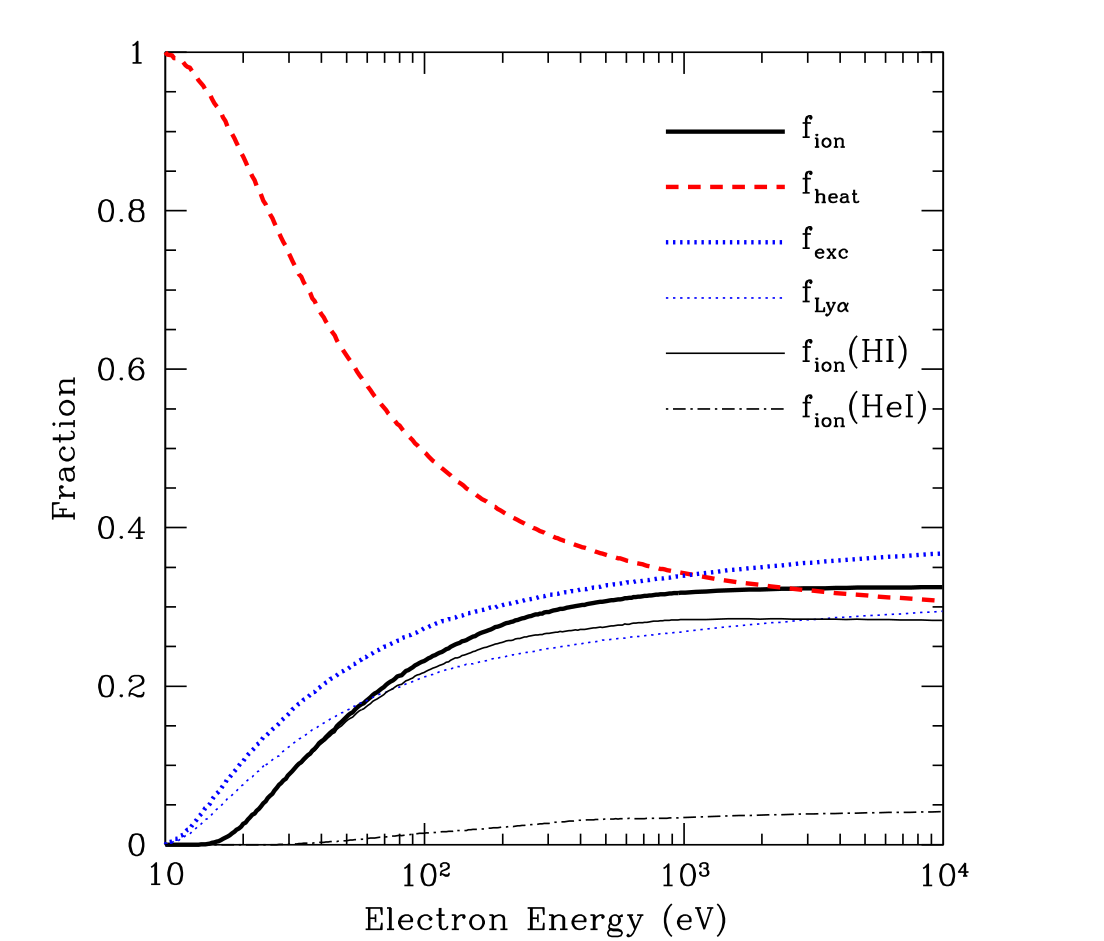
\includegraphics[width=0.60\textwidth]{fig_energy_deposition.png}
\caption[Energy deposition fractions]{\textbf{Why a hard photon is not simply an
ionizing photon.}  Fractions of a fast electron's initial energy deposited as
ionization ($f_{\rm ion}$), heat ($f_{\rm heat}$) and line excitation
($f_{\rm exc}$, with the Ly$\alpha$ part shown separately), for an IGM with
$x_{\rm e}=0.01$.  Below $10.2\,$eV an electron cannot excite or ionize
hydrogen, so \emph{all} its energy becomes heat.  Above $\sim1\,$keV the three
channels split roughly equally and stay flat --- contrary to the naive Bethe
expectation --- because each ionization creates a low-energy secondary that
thermalises.  These are the $f_{\rm heat}$, $f_{\rm ion}$ entering
Eq.~\ref{eq:fheat}, and no statement about the relative ionizing versus heating
power of X-rays or cosmic rays is meaningful without them.
\srcfig{\citet{Furlanetto2009}, Figure 1}}
\label{fig:fheat}
\end{figure}

\subsubsection{Criterion 4 --- the mean free path / SED-hardness criterion}

Because the photoionization cross-section falls steeply with energy
($\sigma\propto E^{-3}$ above threshold), the comoving mean free path of an
X-ray photon rises steeply with energy.  Consequently:
\begin{itemize}[nosep]
  \item Soft X-rays ($\lesssim1\,$keV) are absorbed close to their sources and
        produce \emph{clustered, inhomogeneous} heating.
  \item Hard X-rays ($\gtrsim2\,$keV) free-stream and produce nearly
        \emph{uniform} heating, or escape entirely and contribute to the
        unresolved X-ray background instead.
\end{itemize}
This is why the SED shape, not just the bolometric luminosity, is a criterion in
its own right: \citet{Pacucci2014} show that if the soft band is dominated by
hot-ISM thermal emission rather than by harder X-ray binaries, the large-scale
21-cm power is boosted by roughly a factor of three, and that the \emph{redshift
of the peak} of the large-scale power constrains the X-ray luminosity and host
halo mass while the \emph{amplitude} constrains the soft-band SED, breaking the
degeneracy with bolometric luminosity.  \citet{GesseyJones2023} make the same
argument for cosmic rays, whose heating is short-ranged and therefore leaves
more small-scale power than X-ray heating.


\paragraph{What the spectra actually look like.}
Figure~\ref{fig:seds} makes the criterion concrete: it plots the mean spectrum
of each agent against photon energy, from the H\,\textsc{i} edge to $2\,$keV,
with the three ionization thresholds marked.  The four curves occupy almost
disjoint parts of the spectrum, which is the whole reason the ionizing and
heating budgets decouple.

\begin{itemize}[nosep]
  \item \textbf{Stars} dominate everything by three to seven orders of magnitude
        between $13.6$ and $54.4\,$eV --- and then fall off a cliff.  In the
        words of \citet{Eide2020}, the volume-averaged galaxy spectra ``are
        strongest at H\,\textsc{i} and He\,\textsc{i} ionizing frequencies, and
        fall by orders of magnitude near the He\,\textsc{ii} ionization
        threshold''.  A normal stellar population is therefore an almost
        \emph{monochromatic} source on this scale: it supplies the hydrogen
        budget and essentially nothing else.
  \item \textbf{Nuclear black holes} follow a power law all the way to keV
        energies, which is why they are the only population that reionizes
        helium (Section~\ref{sec:agents}) despite being far too rare to matter
        for hydrogen.
  \item \textbf{Hot ISM} emission is flat to $\sim200\,$eV and then declines;
        \textbf{X-ray binaries} do the opposite, rising to a plateau above
        $\sim500\,$eV.  Below $\sim1\,$keV the two are comparable, which is
        exactly the ambiguity \citet{Pacucci2014} exploit --- see
        Figure~\ref{fig:xraysed}.
\end{itemize}

\begin{figure}[htbp]
\centering
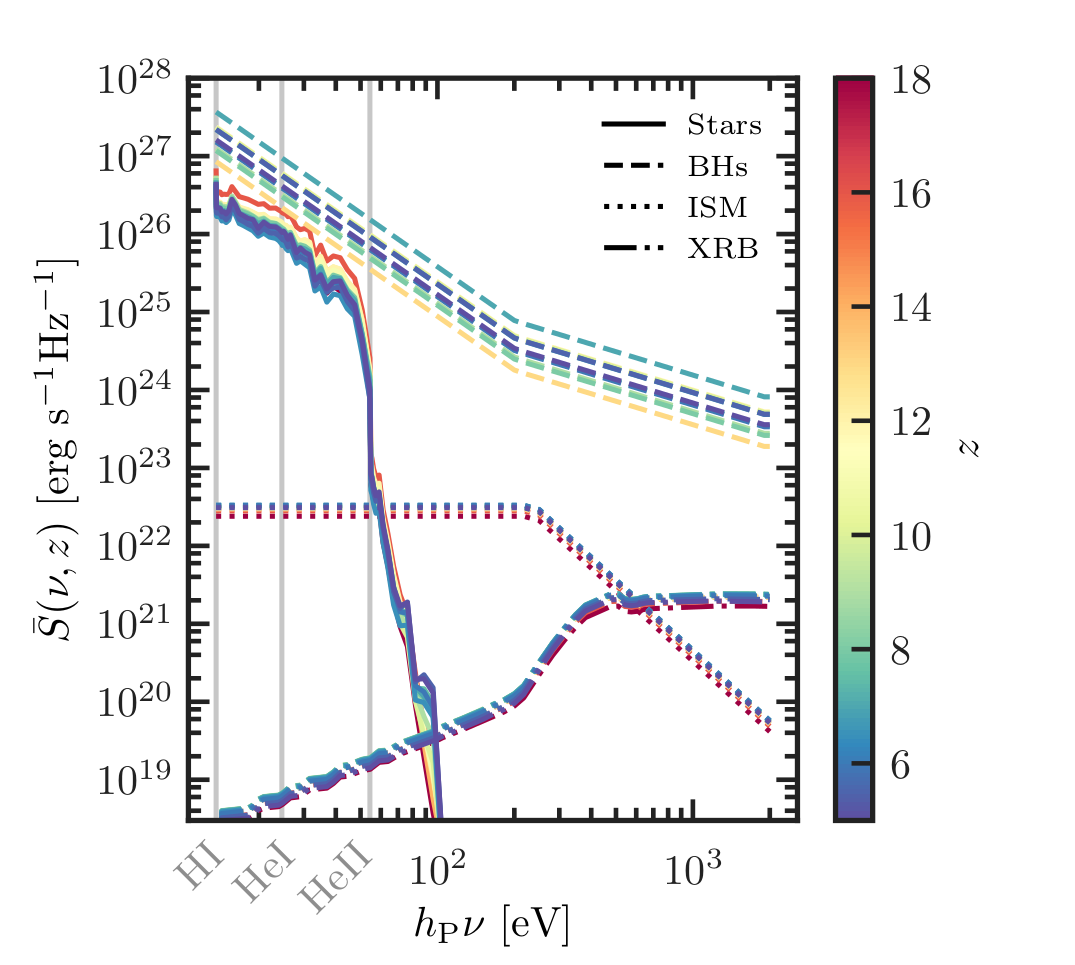
\includegraphics[width=0.72\textwidth]{fig_source_seds.png}
\caption[Emitted spectra of the reionization agents]{\textbf{Where each agent
puts its photons.}  Average spectral energy distribution of stars (solid),
nuclear black holes (dashed), hot ISM (dotted) and X-ray binaries
(dash-dot-dotted) as a function of photon energy, coloured by redshift; grey
vertical lines mark the H\,\textsc{i}, He\,\textsc{i} and He\,\textsc{ii}
thresholds.  Stellar spectra are from BPASS.  Note the near-vertical stellar
drop at $54.4\,$eV: it is the single most important feature on this plot,
because it is why hydrogen and helium reionization are separate events driven
by different populations.
\srcfig{\citet{Eide2020}, Figure 1}}
\label{fig:seds}
\end{figure}

\begin{figure}[htbp]
\centering
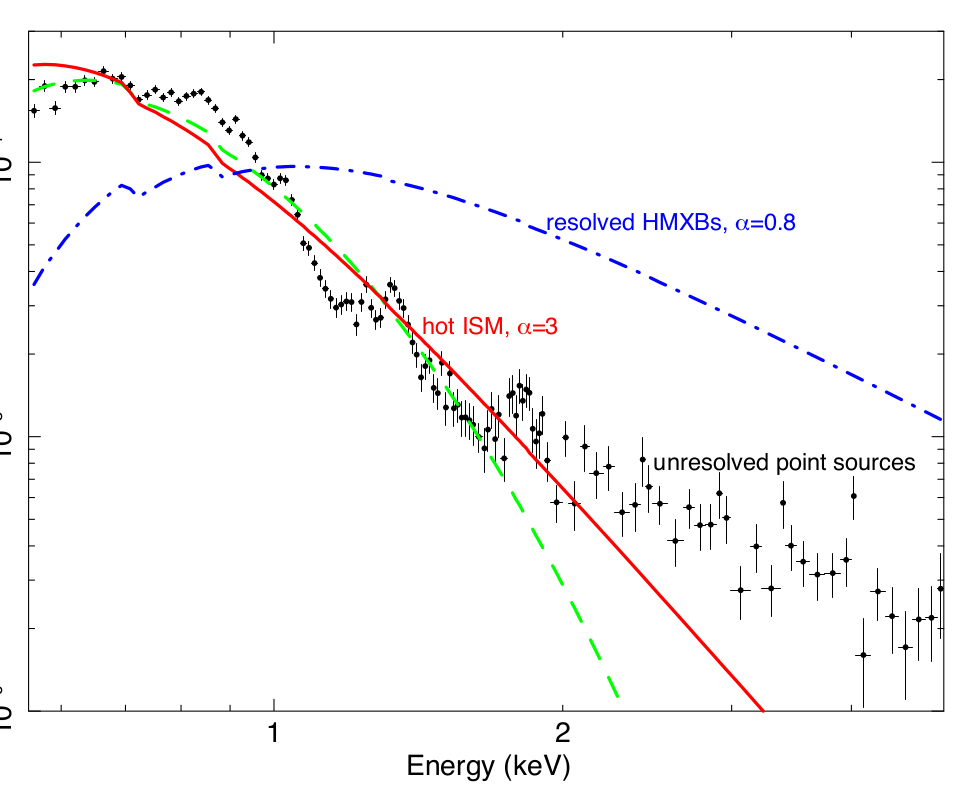
\includegraphics[width=0.62\textwidth]{fig_xray_sed_observed.png}
\caption[Observed soft X-ray SED of star-forming galaxies]{\textbf{The soft
X-ray band, measured rather than assumed.}  Composite \emph{observed} X-ray SED
of 21 local star-forming galaxies, in photons\,cm$^{-2}$\,s$^{-1}$\,keV$^{-1}$.
Below $\sim2\,$keV the emission is dominated by the hot ISM (red solid, a
power law of energy index $\alpha=3$; green dashed, a thermal bremsstrahlung
fit); above $\sim2\,$keV by unresolved point sources, chiefly high-mass X-ray
binaries (blue dot-dashed, $\alpha=0.8$).  All curves include intrinsic
absorption by $N_{\rm HI}\sim2$--$3\times10^{21}\,{\rm cm^{-2}}$.  The two
components have comparable soft-band luminosity per unit SFR but
\emph{dramatically different} spectral shapes --- which is why the split
between them changes the predicted 21-cm power by a factor of three.
\srcfig{\citet{Pacucci2014}, Figure 1}}
\label{fig:xraysed}
\end{figure}

\paragraph{Relative photon abundance by energy band.}
For a source with $\epsilon_\nu\propto\nu^{-\alpha}$ the photon emission rate
per unit frequency is $\dot n_\nu = \epsilon_\nu/h\nu \propto \nu^{-\alpha-1}$,
so the fraction of hydrogen-ionizing photons emitted above an energy $E$ is
just $(E/E_{\rm HI})^{-\alpha}$.  Table~\ref{tab:bands} evaluates this for the
effective ionizing-source index $\alpha_{\rm s}=2.0\pm0.6$ measured by
\citet{Gaikwad2023} and for the AGN power law $\alpha_{\rm AGN}=1.7$ adopted by
\citet{Asthana2024} (who print it as $\alpha=-1.7$ in the $\nu^{+\alpha}$
convention; this document uses $\epsilon_\nu\propto\nu^{-\alpha}$ throughout).  \textbf{These percentages are my own calculation} from
those published indices (script: \texttt{photon\_energy\_fractions.py};
the closed form is verified with \texttt{sympy}), not values quoted in either
paper.

\begin{table}[htbp]
\centering
\caption{Share of hydrogen-ionizing photons by energy band for a power-law
emissivity $\epsilon_\nu\propto\nu^{-\alpha}$.  Thresholds: H\,\textsc{i}
$13.598\,$eV, He\,\textsc{i} $24.587\,$eV, He\,\textsc{ii} $54.418\,$eV.}
\label{tab:bands}
\begin{tabular}{@{}l c c c c@{}}
\toprule
$\alpha$ & source & $13.6$--$24.6$\,eV & $24.6$--$54.4$\,eV & $>54.4$\,eV \\
\midrule
$1.4$ & $\alpha_{\rm s}-1\sigma$ & $56.4\%$ & $29.3\%$ & $14.3\%$ \\
$2.0$ & $\alpha_{\rm s}$ (fiducial) & $69.4\%$ & $24.3\%$ & $6.2\%$ \\
$2.6$ & $\alpha_{\rm s}+1\sigma$ & $78.6\%$ & $18.7\%$ & $2.7\%$ \\
$1.7$ & $\alpha_{\rm AGN}$ & $63.5\%$ & $27.1\%$ & $9.5\%$ \\
\bottomrule
\end{tabular}
\end{table}

\medskip\noindent
\flag{Important caveat, and the reason Figure~\ref{fig:seds} matters more than
Table~\ref{tab:bands}: a single power law is the wrong shape for a stellar
population above the He\,\textsc{ii} edge.  $\alpha_{\rm s}$ is an
\emph{effective} index fitted so that the escaping emissivity reproduces the
Ly$\alpha$ forest over a narrow range above $13.6\,$eV; extrapolating it to
$54.4\,$eV predicts $\sim6\%$ of photons in the He\,\textsc{ii} band, whereas
the BPASS spectra in Figure~\ref{fig:seds} fall by several orders of magnitude
there, putting the true stellar fraction far below $1\%$.  Use the table for
the AGN row and for the $13.6$--$24.6\,$eV split; use the figure for anything
involving the He\,\textsc{ii} edge.}

\subsubsection{Criterion 5 --- calibrated luminosity-to-SFR (or -to-mass) scalings}

Finally, converting a source population into an energy injection rate requires
an empirical scaling: $L_{\rm X}/{\rm SFR}$ for X-ray binaries, the AGN UV
luminosity function for quasars, a cosmic-ray escape efficiency for supernova
remnants.  These are calibrated locally and extrapolated, and the extrapolation
is now testable: HERA excludes the local, metal-enriched $L_{\rm X}$--SFR
relation at $>99\%$ of posterior volume, requiring instead low-metallicity HMXB
models \citep{HERA2022}.  \citet{Dasgupta2026} further show that the
deterministic $L_{\rm X}$--SFR scaling itself breaks down in high-$z$, low-SFR
regions hosting few sources: sampling $L_{\rm X}$ stochastically from an X-ray
luminosity function enhances 21-cm power at $k>0.3\,\cMpc^{-1}$ while leaving
the global signal and large-scale power unchanged.

\subsubsection{Classification convention used in this document}

\textbf{This threshold convention is mine, not a literature standard}, adopted
so that Table~\ref{tab:agents} is unambiguous.  Referring to the total ionizing
photon budget (or total energy injection, for heating):
\emph{dominant} $\;>50\%$; \emph{significant} $\;10$--$50\%$;
\emph{minor} $\;1$--$10\%$; \emph{negligible} $\;<1\%$.
Where a paper states a percentage I use it; where it states only
``dominant''/``negligible'' I reproduce the paper's word and say so.

\subsection{Catalogue of agents}

\subsubsection{Star-forming galaxies: Lyman-continuum photons}

\textbf{Ionization: dominant.}  This is the consensus position of the corpus.
\citet{Robertson2015} showed that the HST UV LF plus $\fesc=0.2$ and
$\log_{10}\xiion=53.14\,[{\rm s^{-1}}/(\Msun{\rm yr^{-1}})]$ simultaneously
match $\tau=0.066\pm0.012$ (the then-current \emph{Planck} value) and the
observed neutrality evolution over $6\lesssim z\lesssim10$, without requiring a
significant $z\gg10$ population.  Radiative-transfer simulations reach the same
conclusion mechanistically: ``stars are the main driver of hydrogen reionization
and consequently of the thermal history of the IGM'' \citep{Eide2020}.

\medskip\noindent
\textbf{Which galaxies, though, is genuinely unsettled.}  Three positions
coexist in the current literature:
\begin{description}[leftmargin=1.6em]
\item[Faint dwarfs dominate.] \citet{Finkelstein2019} find a solution with
  average $\fesc<5\%$ throughout the bulk of the EoR provided galaxies form down
  to the atomic cooling limit and \xiion\ rises towards fainter magnitudes and
  higher $z$; in this model $M_{\rm UV}>-15$ galaxies dominate the emissivity.
  \citet{Atek2023} measure $\log_{10}\xiion/({\rm Hz\,erg^{-1}})=25.80\pm0.14$
  for eight lensed galaxies at $M_{\rm UV}\sim-17$ to $-15$ (down to
  $0.005L^\star$) --- a factor $\sim4$ above the canonical value --- and
  conclude that faint galaxies alone exceed the requirement even for
  $\fesc\sim5\%$.
\item[Bright ``oligarchs'' dominate.] \citet{Naidu2019} require
  $\fesc=0.21^{+0.06}_{-0.04}$ for $M_{\rm UV}<-13.5$ galaxies, propose
  $\fesc\propto\Sigma^{0.4\pm0.1}$ (star-formation surface density), and find
  that $<5\%$ of galaxies with $M_{\rm UV}<-18$ \emph{and} $\log(M_\star/\Msun)>8$
  supply $\gtrsim80\%$ of the budget,
  with faint sources ($M_{\rm UV}>-16$) necessarily relegated to a minor role in
  order to keep \xHI\ high at $z=7$--$8$.
\item[A leaking minority dominates, and the balance evolves.]  The most recent
  direct constraint in the corpus \citep{Giovinazzo2026} fits 1428 JWST/NIRSpec
  spectra at $5<z<10$ with a picket-fence model and finds that
  $\sim20\%$ of sources --- those with $\fesc>10\%$ --- produce $\sim87\%$ of
  the ionizing photons; bright sources ($M_{\rm UV}\sim-20$) dominate at
  $z=5$--$6$, whereas at $z>6$ faint galaxies ($M_{\rm UV}>-18$) contribute
  roughly equally.
\end{description}

\medskip\noindent
\textbf{Stellar physics matters at the factor level.}  Including binary stars in
the stellar population synthesis raises $\fesc$ to $\approx7$--$10\%$, about
$3\times$ the single-star value (the luminosity-weighted average escape fraction
is $8.5\%$ for binaries versus $2.7\%$ for singles, a factor $\approx3.1$), because
the ionizing luminosity declines more slowly with age; in the SPHINX simulations this is the difference between
volumes that are $99.9\%$ ionized by $z\approx7$ and volumes that fail to
reionize by $z=6$ at all \citep{Rosdahl2018}.

\medskip\noindent
\textbf{Heating: dominant for the ionized phase, negligible for the neutral
phase.}  Stellar LyC photons have a short mean free path and deposit their
excess energy inside H\,\textsc{ii} regions, photoheating them to
$\sim1$--$2\times10^4\,$K \citep{Gaikwad2020,Villasenor2021,Eide2020}.  They do
essentially nothing to the gas between H\,\textsc{ii} regions, which is why the
pre-reionization 21-cm signal is a clean probe of the non-stellar agents.

\subsubsection{Population III stars}

\textbf{Ionization: negligible at $z\lesssim10$; potentially dominant only at
$z\gtrsim30$.}  Pop~III stars are individually far more efficient ionizers ---
harder spectra produce $\sim10\times$ more ionizing photons than Pop~II
\citep{Kulkarni2013} --- but the Pop~III era is self-terminating.
\citet{Kulkarni2013} show with a chemically-tracking semi-analytic model that a
single generation self-enriches its host above the critical metallicity
$Z_{\rm crit}=10^{-4}\,Z_\odot$ in $\sim10^{6}\,$yr, so Pop~III stars supply
$\gtrsim50\%$ of ionizing photons only at $z\gtrsim30$ and $<1\%$ at $z=10$;
comparison of the predicted abundance pattern with measured $z\lesssim6$ DLA
abundances bounds the high-mass Pop~III fractional contribution to the
ionization rate at $\lesssim10\%$ at $z=10$.

\medskip\noindent
The per-star ionizing output is now computed from Geneva zero-metallicity models
over $1.7$--$500\,\Msun$ \citep{Murphy2021}: rotation changes ionizing photon
production by up to $25\%$, convective overshooting by $\sim20\%$, and varying
the IMF slope and mass limits by $20$--$30\%$ at fixed population mass.  These
are the systematic uncertainties on any Pop~III budget.

\medskip\noindent
\textbf{Heating: indirect but possibly significant}, via (i) Pop~III supernova
cosmic rays (below) and (ii) Pop~III X-ray binaries \citep{Dasgupta2026}; and
the HERA requirement of low-metallicity HMXB $L_{\rm X}$--SFR scalings
\citep{HERA2022} points in the same direction.

\subsubsection{Quasars and AGN}

\textbf{Hydrogen ionization: contested; most of the corpus says minor to
significant, not dominant.}
\begin{itemize}[nosep]
  \item \citet{Madau2015} constructed the strongest AGN-only case: if the
        claimed abundant faint AGN population at $z=4$--$6$ is real and its
        emissivity persists to $z\sim10$, AGN can reionize hydrogen \emph{and}
        helium with little stellar contribution, giving a flat \GHI\ over
        $2<z<5$, hydrogen fully reionized by $z=5.7$ and $\tau=0.056$.  The
        model predicts helium doubly reionized before $z=4$ and a $50\%$
        He\,\textsc{iii} volume fraction already when hydrogen completes; He
        contributes $\sim13\%$ of $\tau$.
  \item \citet{Kulkarni2018}, from a homogenised sample of $>80{,}000$
        colour-selected AGN from $z=0$ to $7.5$, find the AGN contribution to
        the hydrogen photoionization rate at $z\sim6$ to be
        \emph{sub-dominant, $<3\%$}, rising to $\sim10\%$ only if the LF is
        extrapolated to $M_{1450}=-18$.
  \item \citet{Dayal2020}, with a semi-analytic model of galaxies and black
        holes, find AGN contribute only $10$--$25\%$ of the \emph{cumulative}
        ionizing emissivity by $z=4$ in models that match the reionization
        constraints, with stellar radiation from $M_\star<10^9\,\Msun$ galaxies
        dominating at $z>6$.
  \item \citet{Asthana2024} post-process a Sherwood-Relics simulation with
        radiative transfer and find a ``QSO-assisted'' model (AGN supplying
        $17\%$ of the hydrogen-ionizing emissivity) fits the observed Ly$\alpha$
        optical depth distribution, whereas a QSO-only model does not, and
        overheats the IGM at $z\lesssim5$ through premature He\,\textsc{ii}
        reionization.
  \item \textbf{Dissenting, recent:} \citet{Singha2025} build a unified rest-UV
        AGN LF separating Type~I/Type~II and treating ``little red dots'' and
        X-ray-selected sources as magnitude-filtered subsets of Type~I, and
        anchor the LyC escape fraction to outflow incidence rather than assuming
        quasar-like values.  Integrating over $-27<M_{\rm UV}<-17$ they obtain
        $\dot N_{\rm ion,AGN}=(3.77^{+1.08}_{-0.95})\times10^{51}
        \,{\rm s^{-1}\,\cMpc^{-3}}$ --- nearly twice earlier estimates --- and
        conclude AGN supply $31$--$75\%$ of ionizing photons at $z>5$ for
        $\fesc^{\rm gal}=0.03$--$0.20$, with
        $\Gamma_{\rm HI}\sim(0.5$--$2)\times10^{-12}\,{\rm s^{-1}}$ at
        $z\sim5$--$6$.
        \flag{Note: their quoted $\dot N_{\rm ion,AGN}$ exceeds the total
        measured emissivity $\simeq0.6\times10^{51}\,{\rm s^{-1}\,\cMpc^{-3}}$
        of \citet{Gaikwad2023} by a factor $\sim6$.  I have not reconciled this;
        it may reflect a different definition (emitted vs.\ escaping photons) or
        a genuine inconsistency.  Do not quote both numbers side by side without
        checking the definitions in the papers.}
\end{itemize}

\medskip\noindent
\textbf{Helium ionization: dominant} (Sec.~2.8): AGN are the only population
that supplies $\ge54.4\,$eV photons in quantity
\citep{Eide2020,Kulkarni2018,Madau2015}.

\medskip\noindent
\textbf{Heating: dominant for the post-reionization IGM, negligible for the bulk
neutral IGM.}  Nuclear black holes are rare, so they are negligible for hydrogen
reionization, but they raise local temperatures by $\sim10^4\,$K where they do
ionize helium \citep{Eide2020}; heat input from helium reionization dominates
the thermal balance of the IGM \emph{after} hydrogen reionization
\citep{Madau2015}, consistent with the second \Tzero\ peak measured by
\citet{Villasenor2021}.

\subsubsection{High-mass X-ray binaries}

\textbf{Ionization: negligible.}  \citet{Madau2016} follow compact-binary
evolution with population synthesis calibrated to $z<4$ galaxies and integrate
the rate and energy equations: the XRB contribution to ionization of the bulk
IGM never exceeds an electron fraction of $1\%$.

\medskip\noindent
\textbf{Heating: the leading candidate, and now observationally implicated.}
\begin{itemize}[nosep]
  \item The filtered XRB background peaks between $1$ and $2\,$keV; direct
        He\,\textsc{i} photoionization is the main source of IGM heating; the
        largely neutral gas between H\,\textsc{ii} cavities rises above
        $T_{\rm CMB}$ only at $z<10$, once the H\,\textsc{ii} filling factor
        already exceeds $0.1$ \citep{Madau2016}.  This makes 21-cm
        \emph{emission} a late phenomenon in this scenario.
  \item HERA's $T_{\rm S}$ lower limits establish that the IGM was heated above
        the adiabatic cooling limit at least as early as $z=10.4$, and the
        inferred $L_{\rm X<2\,keV}/{\rm SFR}$ excludes the local relation at
        $>99\%$ of posterior volume, requiring evolved low-metallicity stellar
        populations \citep{HERA2022}.
  \item The deterministic $L_{\rm X}$--SFR scaling is itself an approximation:
        stochastic sampling from an X-ray LF enhances small-scale
        ($k>0.3\,\cMpc^{-1}$) 21-cm power while leaving the global signal
        unchanged \citep{Dasgupta2026}.
\end{itemize}

\subsubsection{Hot interstellar medium (thermal bremsstrahlung, soft X-rays)}

\textbf{Ionization: negligible.  Heating: significant, and possibly the
dominant \emph{soft}-band contributor.}  Chandra observations of nearby
star-forming galaxies show ubiquitous sub-keV thermal ISM emission that
generally dominates the soft X-ray luminosity --- precisely the band that
interacts with the IGM.  \citet{Pacucci2014} show that if the first galaxies'
soft band is ISM-dominated rather than XRB-dominated, IGM temperature
fluctuations are substantially increased and the large-scale 21-cm power is
higher by roughly a factor of three.  \citet{Eide2020} independently find that
the ISM component (and to a lesser extent XRBs) significantly shapes the thermal
and ionization state of the neutral and lowly-ionized hydrogen, and thereby
controls the 21-cm absorption-to-emission transition.

\subsubsection{Cosmic rays}

\textbf{Ionization: minor, and poorly constrained.}  \citet{Tueros2014} simulate
particle cascades in the primordial IGM and argue that cosmic rays accelerated
at the termination shocks of the first microquasar jets could contribute to
reionization \emph{as much as} the X-rays from the same objects' accretion
discs, depending on the electron-to-proton ratio; if the primordial magnetic
field is $\sim10^{-17}\,$G the cosmic rays can ionize material far from the
first stars.  \flag{This is a single-paper, model-dependent claim; it is not
corroborated elsewhere in the corpus.}

\medskip\noindent
\textbf{Heating: potentially significant at cosmic dawn.}
\citet{Sazonov2015} argue that Pop~III supernova remnants can channel a
significant fraction of their kinetic energy into low-energy ($E<30\,$MeV)
cosmic rays that escape into the IGM and heat it by $\sim10$--$100\,$K by
$z\sim15$, \emph{before} X-ray mechanisms take over.  \citet{GesseyJones2023}
build the first 3D semi-numerical model of this channel and find that cosmic-ray
heating is short-ranged, hence clustered around star-forming sites, producing a
sharper contrast between heated (emission) and unheated (absorption) regions and
therefore \emph{more small-scale 21-cm power} than X-ray heating --- an
observational discriminant.  In models where cosmic rays escape efficiently only
from low-mass haloes (as expected for Pop~III remnants), the interplay with
Lyman--Werner feedback can produce a local peak in $T_{\rm K}$ and a flattened
global absorption trough.

\subsubsection{Ly$\alpha$ photons: Wouthuysen--Field coupling, Ly$\alpha$ and CMB heating}

\textbf{Ionization: negligible} (Ly$\alpha$ photons are below the ionization
threshold).  \textbf{Heating: subdominant in general, but decisive for the
interpretation of the 21-cm signal.}  \citet{Reis2021} include Ly$\alpha$
heating, CMB heating mediated by Ly$\alpha$ photons, and multiple Ly$\alpha$
scattering, and find:
\begin{itemize}[nosep]
  \item In models with weak X-ray heating these processes raise the gas
        temperature by up to $\mathcal{O}(100)\,$K.
  \item The global-signal absorption trough acquires a \emph{floor} of
        $-165\,$mK at $z\approx15$--$19$, whereas for a purely adiabatically
        cooling universe the deepest possible absorption is $-178\,$mK at
        $z=19$, $-216\,$mK at $z=15$ and $-264\,$mK at $z=10$.
  \item The maximum possible power at $z=9$, $k=0.1\,{\rm Mpc^{-1}}$ is
        attenuated by a factor $6.6$.
  \item At cosmic dawn the heating terms are subdominant, but multiple
        scattering amplifies the power spectrum by a factor $\sim2$--$5$.
\end{itemize}
Crucially, Ly$\alpha$ photons are what couple $T_{\rm S}$ to $T_{\rm K}$ in the
first place, so \emph{no} 21-cm constraint on any other heating agent exists
without them.

\subsubsection{Secondary electrons (a channel, not a source)}

Not an agent in its own right, but the mechanism through which every
high-energy agent (X-rays, cosmic rays, and any exotic injection) is converted
into ionization, heat and Ly$\alpha$ photons.  \citet{Furlanetto2009} provide
the standard energy-deposition fractions; their key results are summarised in
Section~\ref{sec:criteria} (Criterion 3).  Any statement about the relative
ionizing versus heating power of a hard-photon source is meaningless without
specifying $f_{\rm ion}(E,x_{\rm e})$ and $f_{\rm heat}(E,x_{\rm e})$.

\subsubsection{Structure-formation shocks}

\textbf{Ionization: negligible.  Heating: guaranteed, and dominant before the
first sources switch on.}  Gravitational collapse drives shocks into the IGM
irrespective of any radiative source, so this channel has no free efficiency
parameter --- it is the floor beneath every other heating mechanism.
\citet{Furlanetto2003} extend the Press--Schechter formalism to large-scale
structure shocks and show that \emph{before} reionization the thermal energy of
the IGM is dominated by these shocks rather than by virialised objects; the same
shocks strip $\sim10\%$ of the gas from dark-matter minihaloes, accelerate cosmic
rays (linking to Section~\ref{sec:agents}), and generate a diffuse
inverse-Compton/cooling radiation background \emph{before the first stars form}.

\medskip\noindent
Quantitatively the effect on the observable is modest but not ignorable.
Running high-resolution hydrodynamic simulations of early structure formation
with star formation and feedback switched off, \citet{Xu2021} find that the
combination of non-linear density fluctuations, shock heating and Compton
heating reduces the \emph{maximum} global 21-cm absorption depth by
$\sim15\%$ at $z=17$ relative to a homogeneous or linearly-fluctuating IGM.
This matters directly for claims of anomalously deep absorption: a $15\%$ bias
must be removed before invoking new physics.

\subsubsection{An excess radio background (a background, not a source of energy)}
\label{sec:radio}

\textbf{Ionization: none.  Heating: none --- but it changes every 21-cm
inference.}  This entry is included because it is the principal \emph{degeneracy}
affecting the constraints of Sections~\ref{sec:21cm} and \ref{sec:forest}: since
$\delta T_b \propto (1 - T_{\rm rad}/T_{\rm S})$, an excess radio background at
$1.42\,$GHz mimics a colder IGM, so a 21-cm upper limit that appears to require
heating can instead be satisfied by extra radio photons.

\begin{itemize}[nosep]
  \item \textbf{Phenomenology.}  Assuming a uniform synchrotron-like excess,
        \citet{Fialkov2019} show that it deepens the global signal and
        \emph{enhances} the power spectrum; matching the reported EDGES Low-Band
        feature together with EDGES High-Band, high-$z$ quasar and extragalactic
        radio-background limits requires a star-formation efficiency
        $\ge2.8\%$, a minimum star-forming halo mass
        $M_{\rm h}\lesssim10^{9}\,\Msun$ at $z=17$, and an excess of at least
        $1.9\times$ the CMB at $78\,$MHz (i.e.\ $0.1\%$ of the CMB at
        $1.42\,$GHz).  Notably, the X-ray source properties remain
        \emph{unconstrained} in such models --- which is precisely why this
        degeneracy weakens every heating-agent inference.
  \item \textbf{A candidate physical source.}  \citet{Reis2020} drop the
        uniformity assumption and model an inhomogeneous background from
        high-$z$ radio galaxies.  This introduces a genuinely new type of 21-cm
        fluctuation, alongside density, velocity, Ly$\alpha$ coupling, heating
        and reionization; even a moderately enhanced radio efficiency
        significantly alters the power spectrum in weak-X-ray-heating models,
        and EDGES-compatible models enhance the $z\sim17$ power spectrum by up
        to two orders of magnitude.
  \item \textbf{A strong counter-argument.}  \citet{Sharma2018} points out that
        for the relativistic electrons invoked in these scenarios (accelerated
        by accretion onto SMBHs or by first-star supernovae), the synchrotron or
        inverse-Compton cooling time is at least three orders of magnitude
        shorter than the duration of the EDGES feature, irrespective of magnetic
        field strength; the resulting $1.42\,$GHz emission is $\sim10^3$ times
        smaller than the non-cooling estimate.  On this argument astrophysical
        excess-radio-background scenarios are ``very unlikely''.
\end{itemize}

\noindent
\textbf{Status:} unresolved.  The corpus contains both a viable phenomenology
\citep{Fialkov2019,Reis2020} and a strong energetics objection
\citep{Sharma2018}, and the LOFAR analysis of \citet{Ghara2025} leaves the
radio-background efficiency unconstrained over its full prior at 95\%
credibility.  Every $T_{\rm S}$ or $T_{\rm K}$ limit quoted in this document
should be read as conditional on there being no such background.

\subsection{Summary table of agents}

\begin{longtable}{@{}p{3.4cm} p{3.1cm} p{4.4cm} p{4.0cm}@{}}
\caption{Contribution of each agent to hydrogen ionization and to IGM heating.
Thresholds follow the convention of Section~\ref{sec:criteria}
(dominant $>50\%$, significant $10$--$50\%$, minor $1$--$10\%$,
negligible $<1\%$); words in quotes are the source paper's own.}
\label{tab:agents}\\
\toprule
Agent & H ionization & IGM heating & Key references \\
\midrule
\endfirsthead
\toprule
Agent & H ionization & IGM heating & Key references \\
\midrule
\endhead
\bottomrule
\endfoot
Star-forming galaxies (LyC) &
\textbf{Dominant} &
Dominant for ionized phase ($\sim1$--$2\times10^4$\,K); negligible for neutral IGM &
\citet{Robertson2015,Finkelstein2019,Naidu2019,Atek2023,Giovinazzo2026,Eide2020} \\
\addlinespace
\quad -- bright ``oligarchs'' &
$>80\%$ of budget in one model; contested &
as above &
\citet{Naidu2019,Giovinazzo2026} \\
\addlinespace
\quad -- faint dwarfs &
Dominant in other models; contested &
as above &
\citet{Finkelstein2019,Atek2023} \\
\addlinespace
Population III stars &
\textbf{Negligible} at $z\lesssim10$ ($<1\%$ at $z=10$; $\lesssim10\%$ bound from DLA abundances); $\gtrsim50\%$ only at $z\gtrsim30$ &
Indirect, via Pop~III SN cosmic rays and Pop~III XRBs &
\citet{Kulkarni2013,Murphy2021,Sazonov2015,Dasgupta2026} \\
\addlinespace
Quasars / luminous AGN &
Minor: $<3\%$ of \GHI\ at $z\sim6$ ($\sim10\%$ if LF extended to $M_{1450}=-18$) &
Dominant \emph{after} H reionization, via He\,\textsc{ii} &
\citet{Kulkarni2018,Madau2015,Dayal2020} \\
\addlinespace
Faint AGN / little red dots &
\textbf{Contested}: $17\%$ works, AGN-only fails \citep{Asthana2024}; $31$--$75\%$ claimed \citep{Singha2025} &
Overheats IGM at $z\lesssim5$ if dominant &
\citet{Asthana2024,Singha2025,Dayal2020} \\
\addlinespace
AGN, He\,\textsc{ii} ionization &
\textbf{Dominant} (only viable source of $\ge54.4$\,eV photons) &
\textbf{Dominant}: $+\sim10^4$\,K locally; sets $\Tzero$ peak at $z\sim3$ &
\citet{Eide2020,Kulkarni2018,Villasenor2021,Madau2015} \\
\addlinespace
High-mass X-ray binaries &
\textbf{Negligible} ($x_{\rm e}$ never exceeds $1\%$) &
\textbf{Leading candidate}; requires low-metallicity $L_{\rm X}$/SFR &
\citet{Madau2016,HERA2022,Dasgupta2026} \\
\addlinespace
Hot ISM (soft X-ray bremsstrahlung) &
Negligible &
\textbf{Significant}: can dominate the soft band; $\times3$ large-scale 21-cm power &
\citet{Pacucci2014,Eide2020} \\
\addlinespace
Nuclear BHs / mini-quasars &
Negligible (rare) &
Significant locally; only sources fully ionizing He &
\citet{Eide2020} \\
\addlinespace
Cosmic rays &
Minor / unconstrained; comparable to microquasar X-rays in one model &
Possibly significant at $z\sim15$ ($\Delta T\sim10$--$100$\,K); distinctive small-scale 21-cm signature &
\citet{Sazonov2015,GesseyJones2023,Tueros2014} \\
\addlinespace
Ly$\alpha$ photons (WF, Ly$\alpha$/CMB heating) &
\textbf{Negligible} (sub-threshold) &
Up to $\mathcal{O}(100)$\,K in weak-X-ray models; sets the $-165$\,mK absorption floor; \emph{required} for any 21-cm coupling &
\citet{Reis2021} \\
\addlinespace
Structure-formation shocks &
\textbf{Negligible} &
\textbf{Dominant before the first sources}; reduces max.\ global absorption by $\sim15\%$ at $z=17$ &
\citet{Furlanetto2003,Xu2021} \\
\addlinespace
Secondary electrons &
Channel, not source: $f_{\rm ion}(E,x_{\rm e})$ &
Channel, not source: $f_{\rm heat}(E,x_{\rm e})$; equal three-way split at $1$--$10$\,keV &
\citet{Furlanetto2009} \\
\addlinespace
Excess radio background &
None &
None --- but mimics a cold IGM and so degrades every 21-cm heating constraint; energetics disputed &
\citet{Fialkov2019,Reis2020,Sharma2018,Ghara2025} \\
\addlinespace
Small-scale structure / clumping &
Not a source: a \emph{sink}.  $C\approx12$ observationally vs $C\approx3$ in simulations; $C_{\rm HII,rec}=6.2^{+4.1}_{-2.1}$ required &
Sets the recombination rate and \lmfp\ fluctuations; peak $C=5$--$20$ for $\sim10$\,Myr post-I-front &
\citet{Davies2024,Austin2025,DAloisio2020} \\
\end{longtable}


%=======================================================================
\section{The parameters that govern the reionization history}
\label{sec:params}
%=======================================================================

This section collects the quantities that actually enter a reionization
calculation --- the ones you have to choose a value for before
Eq.~\ref{eq:qdot} can be integrated.  Each parameter gets its own entry: the
symbol and the range it spans across the corpus in the heading, then the
individual determinations behind that range, one per bullet, each with its
source.

\medskip\noindent
Every bullet carries a tag: \tM\ for a value \emph{measured} or inferred from
data, \tA\ for one \emph{assumed} as a model input, \tD\ for one
\emph{derived} here.  The distinction matters --- several of the widest ranges
below are ranges of assumption, not of measurement.  A heading range is the
spread \emph{across} the cited papers, never a confidence interval; where a
single paper's own uncertainty is quoted it appears in the bullet.  Every value
was checked against its source PDF under the audit of Section~\ref{sec:audit}.

%-----------------------------------------------------------------------
\subsection{Source term --- how many ionizing photons escape}
%-----------------------------------------------------------------------

\pheader{\fesc}{Lyman-continuum escape fraction of galaxies}{$0.03$--$0.25$}
\begin{pbullets}
  \item \tA\ $<5\%$ averaged through the bulk of the EoR, in a model where the
        faintest galaxies dominate the emissivity and \xiion\ rises towards
        fainter magnitudes \citep{Finkelstein2019}.
  \item \tA\ $0.21^{+0.06}_{-0.04}$ for $M_{\rm UV}<-13.5$, in the
        bright-galaxy picture, with $\fesc\propto\Sigma_{\rm SFR}^{0.4\pm0.1}$
        \citep{Naidu2019}.
  \item \tM\ $\simeq5\%$ inferred from the UV continuum slope $\beta_{\rm UV}$
        via the low-redshift LzLCS calibration \citep{Austin2025}.
  \item \tM\ $\approx7$--$10\%$ in radiation-hydrodynamic simulations that
        include binary stars --- about $3\times$ the single-star value
        \citep{Rosdahl2018}.
  \item \tA\ $0.03$--$0.20$ spanned as an explicit prior when apportioning the
        budget between galaxies and AGN \citep{Singha2025}.
  \item[$\hookrightarrow$] \emph{Not observable at $z>6$}: the IGM is opaque to
        exactly the photons one would need to detect \citep{Giovinazzo2026}.
        Every value above is an inference.
\end{pbullets}

\pheader{\xiion}{Ionizing photon production efficiency, $\log_{10}$(Hz\,erg$^{-1}$)}{$25.05$--$25.80$}
\begin{pbullets}
  \item \tA\ $25.2$, the canonical pre-JWST value \citep{Robertson2015,Munoz2024}.
  \item \tM\ $25.80\pm0.14$ for eight ultra-faint lensed galaxies at
        $M_{\rm UV}\sim-17$ to $-15$ --- a factor $\sim4$ above canonical
        \citep{Atek2023}.
  \item \tM\ $25.5$--$26.0$ across the JWST-era compilation \citep{Munoz2024}.
  \item \tM\ $-0.006^{+0.019}_{-0.017}M_{\rm UV}+25.05^{+0.39}_{-0.34}$, i.e.\
        \emph{magnitude-independent} and consistent with the canonical HST
        value, from 1721 galaxies \citep{Austin2025}.
  \item \tA\ $25.7$ adopted as an intermediate value \citep{Singha2025}.
\end{pbullets}

\pheader{\xiion}{per unit SFR, $\log_{10}$[s$^{-1}$/($\Msun$\,yr$^{-1}$)]}{$53.14$}
\begin{pbullets}
  \item \tA\ $53.14$, fiducial, paired with $\fesc=0.2$ \citep{Robertson2015}.
\end{pbullets}

\pheader{$\alpha_{\rm UV}$}{UV luminosity function faint-end slope}{$-2.2$ to $-1.7$}
\begin{pbullets}
  \item \tM\ $-2.2\pm0.2$ for star-forming galaxies and $-1.7\pm0.2$ for
        ``smouldering'' ones --- two populations with genuinely different
        slopes \citep{Austin2025}.
\end{pbullets}

\pheader{$M_{\rm UV}^{\rm lim}$}{Faint-end integration limit}{$-17$ to $-11$}
\begin{pbullets}
  \item \tM\ $-17$, the limit of direct observation \citep{Austin2025}.
  \item \tA\ $-13.5$, the common working choice, set by the UVLF turnover in
        Abell~S1063 \citep{Austin2025,Naidu2019}.
  \item \tA\ $-11$, an extrapolation which only worsens the photon budget
        \citep{Munoz2024}.
\end{pbullets}

\pheader{\nion}{Escaping ionizing emissivity (s$^{-1}$\,cMpc$^{-3}$)}{$\simeq(0.3$--$0.7)\times10^{51}$}
\begin{pbullets}
  \item \tM\ $\simeq0.6\times10^{51}$, remarkably flat across
        $4.9\le z\le6.0$, from forward-modelling the Ly$\alpha$ forest
        \citep{Gaikwad2023}.
  \item \tM\ $\log_{10}=50.31^{+0.07}_{-0.06}$ for $M_{\rm UV}<-17$ from
        JWST/NIRCam \citep{Austin2025}.
  \item[$\hookrightarrow$] \tD\ Equivalent to $3.4$ ionizing photons per
        hydrogen atom per Gyr (Section~\ref{sec:crosscheck}), against
        $\approx3$ photons per baryon required at $C\approx12$
        \citep{Davies2024}.
\end{pbullets}

\pheader{$f_\star$}{Star-formation efficiency}{$\ge2.8\%$}
\begin{pbullets}
  \item \tM\ $\ge2.8\%$, a lower limit from matching the EDGES-era global
        signal together with high-$z$ quasar and radio-background limits
        \citep{Fialkov2019}.
\end{pbullets}

\pheader{$M_{\rm min}$}{Minimum star-forming halo mass}{$10^{9}$--$10^{9.4}\,\Msun$}
\begin{pbullets}
  \item \tM\ $\gtrsim2.6\times10^{9}\,\Msun[(1{+}z)/10]^{1/2}$, equivalently
        $V_{\rm c}\gtrsim50$\,km\,s$^{-1}$ (95\% credibility), from the joint
        21-cm + Lyman-line + CMB fit \citep{Sims2025}.
  \item \tA\ $\log M_{\rm h}\sim9$ as the photosuppression mass during and
        after reionization \citep{Finkelstein2019}.
  \item \tM\ $\lesssim10^{9}\,\Msun$ at $z=17$, an upper limit from the
        excess-radio-background fit \citep{Fialkov2019}.
\end{pbullets}

%-----------------------------------------------------------------------
\subsection{Source term --- the AGN contribution}
%-----------------------------------------------------------------------

\pheader{$f_{\rm AGN}$}{AGN share of the hydrogen-ionizing budget}{$<3\%$ to $75\%$}
\begin{pbullets}
  \item \tM\ $<3\%$ of $\GHI$ at $z\sim6$, rising to $\sim10\%$ only if the
        luminosity function holds to $M_{1450}=-18$, from a homogenised sample
        of $>80{,}000$ AGN \citep{Kulkarni2018}.
  \item \tM\ $10$--$25\%$ of the cumulative emissivity by $z=4$ in models that
        match the reionization constraints \citep{Dayal2020}.
  \item \tM\ $17\%$ works: a QSO-assisted model fits the observed Ly$\alpha$
        optical-depth distribution, while a QSO-only model does not
        \citep{Asthana2024}.
  \item \tM\ $31$--$75\%$ at $z>5$ claimed from a unified rest-UV AGN
        luminosity function \citep{Singha2025} --- \emph{disputed}; see the
        emissivity flag in Section~\ref{sec:agents}.
\end{pbullets}

\pheader{$\beta_{\rm AGN}$}{AGN luminosity function faint-end slope}{$-2.4$ to $-1.7$}
\begin{pbullets}
  \item \tM\ Steepens from $-1.7$ at $z<2.2$ to $-2.4$ at $z\simeq6$
        \citep{Kulkarni2018}.
\end{pbullets}

\pheader{$\alpha_{\rm AGN}$}{AGN ionizing spectral index, $\epsilon_\nu\propto\nu^{-\alpha}$}{$1.7$}
\begin{pbullets}
  \item \tA\ $1.7$, adopted as the AGN power law in radiative-transfer
        post-processing \citep{Asthana2024}.  That paper prints it as
        $\alpha=-1.7$ in the $\nu^{+\alpha}$ convention; this document uses
        $\epsilon_\nu\propto\nu^{-\alpha}$ throughout, so a larger $\alpha$ is
        a \emph{softer} spectrum.
\end{pbullets}

\pheader{$t_{\rm Q}$}{Quasar lifetime}{$10^{3}$--$10^{8}$\,yr}
\begin{pbullets}
  \item \tM\ $\lesssim7$\,Myr across all redshift bins, fitted jointly with
        \xHI\ from stacked damping wings \citep{Durovcikova2024}.
  \item \tA\ $10^{3}\le t_{\rm Q}\le10^{8}$\,yr marginalised over when
        extracting \xHI\ from individual quasars \citep{Davies2018}.
  \item \tA\ $10$\,Myr assumed for every AGN in the simulation
        \citep{Asthana2024}.
\end{pbullets}

%-----------------------------------------------------------------------
\subsection{Sink term --- where the photons go}
%-----------------------------------------------------------------------

\pheader{$C_{\rm HII}$}{Clumping factor, $\langle n_{\rm H}^2\rangle/\langle n_{\rm H}\rangle^2$}{$3$ to $\approx12$}
\begin{pbullets}
  \item \tA\ $3$, the long-standing fiducial \citep{Robertson2015}.
  \item \tM\ Peaks at $5$--$20$ about $10$\,Myr after the ionization front
        passes and relaxes to $\approx3$ only by $300$\,Myr; un-relaxed gas
        boosts total recombinations by $\approx50\%$ \citep{DAloisio2020}.
  \item \tM\ $6.2^{+4.1}_{-2.1}$ \emph{required} for stable reionization at
        $z\simeq6$ when the UVLF is extrapolated to $M_{\rm UV}=-13.5$
        \citep{Austin2025}.
  \item \tM\ $\approx12$ globally, from imposing ionization equilibrium on the
        measured \lmfp\ and \GHI\ --- four times the simulation value, and
        worth $\approx3$ photons per baryon \citep{Davies2024}.
\end{pbullets}

\pheader{\lmfp}{Mean free path of Lyman-continuum photons}{$0.75$--$9.09$\,pMpc}
\begin{pbullets}
  \item \tM\ $9.09^{+1.62}_{-1.28}$\,pMpc at $z=5.1$ (68\% confidence), on the
        low-redshift power-law extrapolation \citep{Becker2021}.
  \item \tM\ $0.75^{+0.65}_{-0.45}$\,pMpc at $z=6.0$ --- a factor $\sim7$
        \emph{below} that extrapolation; neglecting the quasar proximity effect
        biases it high by a factor $\ge2$ \citep{Becker2021}.
  \item \tM\ $8.3$--$57$\,$h^{-1}$\,cMpc over $6.0\ge z\ge4.9$, marginalised
        over $\GHI$ and the thermal parameters \citep{Gaikwad2023}.
\end{pbullets}

\pheader{$\alpha_{\rm B}$}{Case-B recombination coefficient}{$1.43$--$2.59\times10^{-13}$\,cm$^3$\,s$^{-1}$}
\begin{pbullets}
  \item \tA\ $2.59\times10^{-13}$\,cm$^3$\,s$^{-1}$ at $T=10^{4}$\,K and
        $1.43\times10^{-13}$ at $T=2\times10^{4}$\,K --- the temperature
        \citet{Robertson2015} adopt.  Tabulated values from Osterbrock \&
        Ferland (2006), Table~2.1, a textbook and not part of the corpus.
  \item[$\hookrightarrow$] Case B excludes recombinations directly to the
        ground state, which emit another ionizing photon and so cause no net
        change; the choice alone is worth $\sim40\%$ against case~A.
\end{pbullets}

\pheader{$t_{\rm rec}$}{IGM recombination time at $z=7$}{$704$--$2113$\,Myr}
\begin{pbullets}
  \item \tD\ $704$\,Myr for $C_{\rm HII}=3$ and $2113$\,Myr for
        $C_{\rm HII}=1$, at $T=2\times10^{4}$\,K
        (Section~\ref{sec:crosscheck}).  The factor $3$ in $C_{\rm HII}$ maps
        directly onto the recombination sink.
\end{pbullets}

%-----------------------------------------------------------------------
\subsection{The resulting history}
%-----------------------------------------------------------------------

\pheader{$\tau$}{CMB Thomson optical depth}{$0.054$--$0.067$}
\begin{pbullets}
  \item \tM\ $0.054\pm0.007$ (68\% CL), TT,TE,EE+lowE+lensing
        \citep{Planck2018}.
  \item \tM\ $0.0566^{+0.0053}_{-0.0062}$ from large-scale polarization alone
        and $0.059\pm0.006$ combined, with improved HFI map-making
        \citep{Pagano2019}.
  \item \tM\ $0.067\pm0.011$ from an astrophysics-anchored fit that excludes
        large-scale CMB polarization \citep{MonteroCamacho2026}.
\end{pbullets}

\pheader{$z_{50}$}{Mid-point, $\xHI=0.5$}{$6.9$--$8.1$}
\begin{pbullets}
  \item \tM\ $7.16^{+0.15}_{-0.12}$ from the joint 21-cm + Lyman-line + CMB
        analysis \citep{Sims2025}.
  \item \tM\ $6.9<z<7.6$ from quasar absorption \citep{Fan2022}.
  \item \tA\ $8.14\pm0.61$ --- but this is a \emph{tanh-model} quantity, not a
        direct measurement \citep{Pagano2019}.
\end{pbullets}

\pheader{$z_{\rm end}$}{Completion redshift}{$5.2$--$5.3$}
\begin{pbullets}
  \item \tM\ Homogeneous-UVB models ruled out at $z\ge5.4$ ($>3.5\sigma$) from
        67 quasar sightlines \citep{Bosman2021}.
  \item \tM\ Long dark gaps persist to $z\simeq5.3$ \citep{Zhu2021}.
  \item \tM\ Radiative-transfer modelling of \GHI, \lmfp\ and $\xHI$ favours
        completion by $z\simeq5.2$ \citep{Gaikwad2023}.
\end{pbullets}

\pheader{$\Delta z_{\rm re}$}{Duration}{$<1.8$ to $<4.2$}
\begin{pbullets}
  \item \tM\ $<1.8$ (95\% credibility) from 21-cm + Lyman-line + CMB
        \citep{Sims2025}.
  \item \tM\ $1.0^{+1.6}_{-0.7}$, and $<4.1$ at 95\% confidence, from the
        first $\ge3\sigma$ kSZ detection \citep{Reichardt2020}.
  \item \tM\ $\Delta^{50}z_{\rm re}<4.2$ (95\%) from SPT-3G, measured between
        ionized fractions of 25\% and 75\% --- a different interval from the
        row above, so the two limits are not directly comparable
        \citep{Chaubal2026}.
\end{pbullets}

\pheader{$\GHI$}{H\,\textsc{i} photoionization rate}{$(0.145$--$0.557)\times10^{-12}$\,s$^{-1}$}
\begin{pbullets}
  \item \tM\ Falls from $0.557^{+0.376}_{-0.218}\times10^{-12}$\,s$^{-1}$ at
        $z=5.0$ to $0.145^{+0.157}_{-0.087}\times10^{-12}$\,s$^{-1}$ at
        $z=6.0$ --- only a factor $\sim4$, far less than the four orders of
        magnitude in $\xHI$ over the same interval, because the collapse is
        driven by \lmfp\ rather than by the sources \citep{Gaikwad2023}.
\end{pbullets}

%-----------------------------------------------------------------------
\subsection{Thermal state and heating agents}
%-----------------------------------------------------------------------

\pheader{\Tzero}{Ionized IGM temperature at mean density}{$(1.05$--$1.4)\times10^{4}$\,K}
\begin{pbullets}
  \item \tM\ $11000\pm1600$, $10500\pm2100$ and $12000\pm2200$\,K at
        $z=5.4$, $5.6$, $5.8$, from transmission-spike widths
        \citep{Gaikwad2020}.
  \item \tM\ Two peaks: $1.3\times10^{4}$\,K when hydrogen reionization
        completes near $z\sim6$, and $1.4\times10^{4}$\,K when
        He\,\textsc{ii} completes near $z\sim3$ \citep{Villasenor2021}.
  \item[$\hookrightarrow$] Measures the \emph{ionized} phase only.  Never plot
        it on the same curve as $T_{\rm S}$.
\end{pbullets}

\pheader{$T_{\rm S}$}{Spin temperature of the neutral IGM}{$>6$--$11$\,K}
\begin{pbullets}
  \item \tM\ $>11.0$\,K at $z=7.9$ and $>6.2$\,K at $z=10.4$ (95\% credibility;
        $>35.2$ and $>26.4$\,K at 68\%), ruling out cold reionization
        \citep{HERA2022}.
\end{pbullets}

\pheader{$\langle T_{\rm HI}\rangle$}{Kinetic temperature of the neutral IGM}{$\gtrsim27$\,K}
\begin{pbullets}
  \item \tM\ Models with $\langle T_{\rm HI}\rangle\lesssim27$\,K at
        $z\approx5.6$ for $\xHI=0.1$ are disfavoured at 68\% credibility, from
        a null detection of the 21-cm forest \citep{Soltinsky2026}.
\end{pbullets}

\pheader{$L_{\rm X<2\,keV}/{\rm SFR}$}{X-ray heating efficiency, erg\,s$^{-1}$($\Msun$\,yr$^{-1}$)$^{-1}$}{$10^{39.9}$--$10^{41.8}$}
\begin{pbullets}
  \item \tM\ $10^{39.9}$--$10^{41.6}$ (68\% HPD), tightening to
        $10^{40.4}$--$10^{41.8}$ at 95\%.  More than 99\% of the posterior
        excludes the local, metal-enriched relation, requiring
        low-metallicity high-mass X-ray binaries \citep{HERA2022}.
\end{pbullets}

\pheader{$f_{\rm heat}$}{Fraction of fast-electron energy deposited as heat}{$1/3$ to $1$}
\begin{pbullets}
  \item \tD\ $\to1$ below $10.2$\,eV, where an electron can neither excite nor
        ionize hydrogen; $\approx1/3$ at $1$--$10$\,keV, where heating,
        ionization and excitation split roughly equally; strongly dependent on
        $x_{\rm e}$ and almost independent of density
        \citep{Furlanetto2009}.
\end{pbullets}

\pheader{$\Delta T_{\rm CR}$}{Cosmic-ray heating}{$\sim10$--$100$\,K}
\begin{pbullets}
  \item \tA\ $\sim10$--$100$\,K by $z\sim15$ from sub-relativistic
        ($E<30$\,MeV) cosmic rays escaping Pop~III supernova remnants
        \citep{Sazonov2015}.
\end{pbullets}

\pheader{$\Delta T_{{\rm Ly}\alpha}$}{Ly$\alpha$ + CMB heating}{up to $\mathcal{O}(100)$\,K}
\begin{pbullets}
  \item \tA\ Up to $\mathcal{O}(100)$\,K in models with weak X-ray heating,
        raising the global-signal absorption floor to $-165$\,mK
        \citep{Reis2021}.
\end{pbullets}

\pheader{$A_{\rm r}$}{Excess radio background}{$\ge1.9\times$ CMB at $78$\,MHz}
\begin{pbullets}
  \item \tA\ $\ge1.9\times$ the CMB at $78$\,MHz, equivalently $0.1\%$ of the
        CMB at $1.42$\,GHz, if the EDGES feature is to be explained
        \citep{Fialkov2019}.  Energetically disputed \citep{Sharma2018} and
        observationally unconstrained over its full prior \citep{Ghara2025}.
\end{pbullets}

%-----------------------------------------------------------------------
\subsection{Cosmological inputs (held fixed)}
%-----------------------------------------------------------------------

\pheader{---}{Cosmology}{Planck 2018}
\begin{pbullets}
  \item \tM\ $\Omega_{\rm b}h^2=0.02237\pm0.00015$; $h=0.6736$ (from
        $H_0=67.36\pm0.54$\,km\,s$^{-1}$\,Mpc$^{-1}$); $Y_{\rm p}=0.2454$
        \citep{Planck2018}.
  \item \tD\ $\langle n_{\rm H}\rangle=1.895\times10^{-7}$\,cm$^{-3}$ comoving,
        and $n_{\rm He}/n_{\rm H}=0.0813$ (Section~\ref{sec:crosscheck}).
\end{pbullets}

%-----------------------------------------------------------------------
\subsection{Reading these numbers: the degeneracies}
\label{sec:degeneracies}
%-----------------------------------------------------------------------

The parameters above are not independent, and the degeneracies are what make
reionization hard.  Quoting any one of them without saying which values of the
others were assumed alongside it is close to meaningless.  Nine are stated
explicitly in the corpus:

\begin{enumerate}[leftmargin=1.7em]

\item \textbf{$\fesc\times\xiion$ --- the ionizing budget.}  Only the product
  sets the timing: ``increasing $\xiion$ per galaxy while decreasing $\fesc$
  will yield identical effects on the IGM'', so the two are ``at face value,
  fully degenerate'' \citep{Munoz2024}.  Direct Balmer-line measurements of
  $\xiion$ break it partially; clustering of reionization bubbles, e.g.\ with
  21-cm, is what would break it fully.

\item \textbf{$A_{\rm s}\leftrightarrow\tau$ --- the CMB's own degeneracy.}
  High-$\ell$ CMB spectra measure the combination $A_{\rm s}e^{-2\tau}$, so
  $\delta A_{\rm s}/A_{\rm s}=2\,\delta\tau$ \citep{Pagano2019}.  Large-scale
  polarization is the \emph{only} thing that breaks it and delivers $\tau$
  directly --- which is precisely why excluding low-$\ell$ EE data sends $\tau$
  to $\sim0.09$ and destabilises the cosmology
  \citep{MonteroCamacho2026}.  Planck quote
  $A_{\rm s}e^{-2\tau}=(1.884\pm0.012)\times10^{-9}$ \citep{Planck2018}.

\item \textbf{$C_{\rm HII}\leftrightarrow$ source term.}  Clumping enters only
  through $t_{\rm rec}$, so it trades directly against \nion.  Going from
  $C=3$ to $C\approx12$ demands roughly twice as many ionizing photons
  \citep{Davies2024}, which is why the clumping dispute and the
  photon-budget crisis are the same argument seen from two ends
  \citep{Austin2025}.

\item \textbf{$\GHI\leftrightarrow\lmfp$.}  The forest constrains the product,
  not either alone: ``it is important to vary both $\lambda_{\rm mfp,HI}$ and
  $\langle\Gamma_{\rm HI}\rangle$'' when matching the $\tau_{\rm eff}$
  distribution, and the quoted $\GHI$ errors are ``larger and more realistic''
  precisely because they are marginalised over \lmfp\ \citep{Gaikwad2023}.
  There is a third axis: $\GHI$ is also degenerate with the thermal parameters,
  which is why spike \emph{widths} rather than depths are used to isolate
  $T_0$ \citep{Gaikwad2020}.

\item \textbf{$\xHI\leftrightarrow t_{\rm Q}$ (damping wings).}  Quantitative
  constraints are ``challenging due to \dots\ degeneracies with quasar
  lifetime'' \citep{Davies2018}; both papers using this probe therefore fit
  \xHI\ and $t_{\rm Q}$ \emph{jointly} \citep{Durovcikova2024}.

\item \textbf{$\xHI\leftrightarrow R_{\rm b}$ (bubble size).}  In JWST galaxy
  damping wings the two are correlated because strong Ly$\alpha$ emission can
  mimic high transmission and hence a large ionized bubble, ``which leads to
  the degeneracy between the two parameters and the large uncertainty''
  \citep{Umeda2023}.

\item \textbf{$A_{\rm r}\leftrightarrow f_{\rm X}$ --- radio background versus
  X-ray heating.}  Both set the depth of the 21-cm absorption feature, so they
  are degenerate \citep{Fialkov2019}; and $f_{\rm X}$ is in turn degenerate
  with $f_\star$, since X-ray heating and the Ly$\alpha$ background scale
  together \citep{Reis2021}.  This is why every $T_{\rm S}$ limit in
  Section~\ref{sec:21cm} is conditional, and why the radio-background
  efficiency remains unconstrained over its whole prior \citep{Ghara2025}.
  Cosmic-ray heating joins the same tangle: its 21-cm signature ``may be
  degenerate with those of other physical processes''
  \citep{GesseyJones2023}.

\item \textbf{Dark matter mass $\leftrightarrow$ heating history.}  In the
  21-cm forest, small-scale power is suppressed both by warm dark matter and by
  early heating, and the two ``are degenerate''; the 1D power spectrum is
  proposed specifically to break it \citep{Shao2023}.

\item \textbf{tSZ $\leftrightarrow$ kSZ $\leftrightarrow$ CIB.}  The
  tSZ--CIB correlation is ``partially degenerate with the tSZ and kSZ power''
  \citep{Reichardt2020}, with ``clear degeneracies between all three
  parameters'' \citep{Chaubal2026}.  Since $\Delta z_{\rm re}$ is inferred from
  the patchy kSZ amplitude after subtracting an \emph{assumed} homogeneous
  component, the duration constraint inherits all of it.

\end{enumerate}

\noindent
Three further couplings are worth knowing because they sit inside the
simulations rather than in the fits: \fesc\ is degenerate with the star
formation history \citep{Giovinazzo2026}, with the SFR and the stellar IMF
\citep{Eide2020}, and with the feedback efficiency, ``a natural outcome of the
regulation of $\fesc$ by feedback'' \citep{Rosdahl2018}.  A quoted \fesc\ is
therefore a statement about a whole galaxy-formation model, not a property of
galaxies.

%=======================================================================
\section{Tensions and caveats worth carrying into the paper}
\label{sec:tensions}
%=======================================================================

\begin{enumerate}[leftmargin=1.6em]
\item \textbf{The photon budget crisis} (Figure~\ref{fig:budget}).  Taking
  JWST \xiion\ values and abundances at face value, the \emph{already observed} galaxies
  ($M_{\rm UV}<-15$) not only can drive reionization but would end it too
  early, in tension with the CMB $\tau$ and the Ly$\alpha$ forest; extending to
  $M_{\rm UV}\approx-11$ makes it worse \citep{Munoz2024}.  Proposed
  resolutions in the corpus: a milder \xiion$(z,M_{\rm UV})$ evolution with two
  populations separated by burstiness, which for $M_{\rm UV}\in[-20,-16]$ and a
  reasonable \fesc\ reproduces the $z\lesssim6$ Ly$\alpha$ forest without
  overshooting \citep{Simmonds2024}; and a leaking-minority picture in which
  $\sim20\%$ of galaxies produce $\sim87\%$ of the escaping photons
  \citep{Giovinazzo2026}.
\begin{figure}[htbp]
\centering
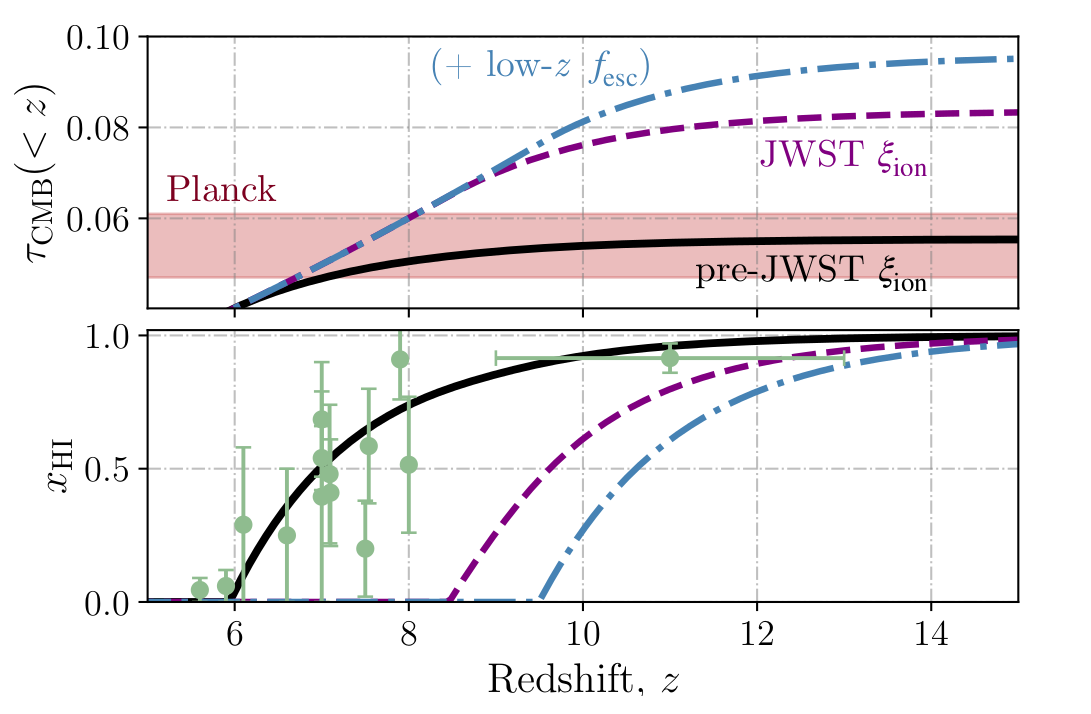
\includegraphics[width=0.66\textwidth]{fig_photon_budget.png}
\caption[The photon budget crisis]{\textbf{The photon budget crisis.}  Bottom:
the neutral fraction $x_{\rm HI}(z)$ for a pre-JWST model (black solid,
$M_{\rm UV}^{\rm cut}=-13$, $\fesc=0.2$), for the same model with a
JWST-calibrated $\xiion$ (purple dashed), and additionally with an $\fesc$ from
low-$z$ analogues (blue dot-dashed); green points are the observational
compilation.  Top: the corresponding cumulative CMB optical depth against the
\emph{Planck} band (red).  Taken at face value the JWST-calibrated models end
reionization far too early and overshoot $\tau$ --- the tension that
Sections~\ref{sec:clumping} and \ref{sec:tensions} discuss.
\srcfig{\citet{Munoz2024}, Figure 1}}
\label{fig:budget}
\end{figure}

\item \textbf{$\tau$ and its cosmological knock-on.}  Excluding large-scale CMB
  polarization weakens the dynamical-dark-energy preference but pushes
  $\tau_{\rm reio}$ up to $\sim0.09$; anchoring on astrophysical \xHI\ data
  instead recovers $\tau_{\rm reio}=0.067\pm0.011$ and restores a
  $\gtrsim2\sigma$ dynamical-dark-energy preference \citep{MonteroCamacho2026}.
  Reionization is thus no longer only an astrophysics problem.
\item \textbf{\fesc\ is not measurable at $z>6$} \citep{Giovinazzo2026}; every
  quoted value is a model inference, and models disagree by factors of a few
  ($<5\%$ in \citet{Finkelstein2019} versus $0.21$ in \citet{Naidu2019}).
\item \textbf{Simulation systematics dominate damping-wing \xHI.}  ATON versus
  CROC shift \xHI\ at $\langle z\rangle=6.46$ from $0.21$ to $0.57$
  \citep{Durovcikova2024}.
\item \textbf{Bubble-size selection bias.}  Bright galaxies sit in merged,
  atypically large ionized bubbles, up to a few dex above the cosmic average at
  the same \xHI\ \citep{Umeda2023}.
\item \textbf{21-cm limits are exclusions of extremes, not measurements.}  The
  LOFAR-disfavoured models are ``extreme ones \dots\ mainly driven by rare and
  large ionized or heated regions'', and the excess-radio-background parameter
  remains unconstrained over its full prior at 95\% \citep{Ghara2025}.
\item \textbf{$\Tzero$ from the forest and $T_{\rm S}$ from 21-cm are not the
  same quantity} (ionized versus neutral phase); they should never be plotted on
  the same thermal-history curve without saying so.
\item \textbf{An unreconciled numerical discrepancy} between the AGN emissivity
  of \citet{Singha2025} and the total measured emissivity of
  \citet{Gaikwad2023} --- see the flag in Section~\ref{sec:agents}.
\item \textbf{The clumping factor is discrepant at the factor-of-4 level}
  between the observational estimate $C\approx12$ \citep{Davies2024} and the
  $C\approx3$ relaxed value of radiation-hydrodynamic simulations
  \citep{DAloisio2020,Robertson2015}.  This is not a detail: it is worth a
  factor $\approx2$ in the required ionizing output, i.e.\ comparable in size
  and opposite in sign to the JWST \xiion\ excess.  \citet{Austin2025}
  argue the two cancel.
\item \textbf{\xiion\ itself is not settled.}  \citet{Atek2023} report
  $\log_{10}\xiion = 25.80\pm0.14$ for ultra-faint lensed galaxies, whereas
  \citet{Austin2025}, from a much larger stellar-mass-complete NIRCam sample,
  find $\approx 25.05^{+0.39}_{-0.34}$ with \emph{no} dependence on
  $M_{\rm UV}$ --- consistent with the canonical HST value.  The photon budget
  crisis is partly a disagreement about this one number.
\item \textbf{Can stellar populations make He\,\textsc{ii}-ionizing photons?}
  The textbook answer is no, and the global budget does not need them to.  But
  He\,\textsc{ii}\,$\lambda1640$ is now detected with high equivalent width at
  $z=8.16$ and $z=10.6$ \citep{Wang2022,Maiolino2026}, the latter with no metal
  lines at all, and rotating Pop~III models can reach the required hardness
  \citep{Wasserman2025}.  Meanwhile the simulations that report stars
  contributing nothing to He\,\textsc{iii} adopt single-star spectral libraries
  \citep{Eide2020}.  Whether this is a genuine stellar contribution, an
  accreting black hole, or shocks is unresolved --- the same ambiguity that
  attended CR7 --- and it matters for \emph{when} He\,\textsc{ii} reionization
  starts, though not for who finishes it.
\item \textbf{Every 21-cm temperature limit is conditional on there being no
  excess radio background} (Section~\ref{sec:radio}), a scenario that is
  phenomenologically viable \citep{Fialkov2019,Reis2020}, energetically
  disputed \citep{Sharma2018}, and observationally unconstrained
  \citep{Ghara2025}.
\end{enumerate}

%=======================================================================
\section{Flagged for your decision (not included on my own judgement)}
\label{sec:flagged}
%=======================================================================

Per your instruction not to decide unilaterally, the following aspects and
caveats surfaced during the search and are still \emph{not} covered by the
corpus.  Each would require adding papers to the folders.

\medskip\noindent
\textbf{Resolved in this revision.}  Four topics previously listed here have now
been incorporated at your request, with 12 papers added
(\texttt{Agents/} 25\,$\to$\,32, \texttt{Constraints/} 20\,$\to$\,25):
the excess radio background (Section~\ref{sec:radio});
the clumping factor and small-scale structure (Section~\ref{sec:clumping});
structure-formation shock heating (Section~\ref{sec:agents});
the 21-cm forest (Section~\ref{sec:forest});
and kSZ patchy-reionization constraints (Section~\ref{sec:ksz}).

\medskip\noindent
\textbf{Still outstanding, awaiting your decision:}

\begin{enumerate}[leftmargin=1.6em]
\item \textbf{Exotic energy injection as a heating/ionizing agent}: dark matter
  annihilation and decay, primordial black hole accretion and evaporation, and
  fuzzy/warm dark matter effects on the source population.  You declined this in
  the first round; note that it now touches the document in two places anyway
  --- \citet{Shao2023} motivate the 21-cm forest power spectrum precisely as a
  way to break the warm-dark-matter/heating degeneracy, and
  \citet{Fialkov2019} note that the X-ray source properties are unconstrained in
  excess-radio-background models.  If you later want the agent catalogue to be
  exhaustive rather than astrophysical-only, this is the remaining gap.
\item \textbf{Gamma-ray bursts} as both probes of \xHI\ and (marginally) as
  sources.
\item \textbf{Metal absorption lines and the CGM} during the EoR as a
  complementary probe (mentioned in \citet{Fan2022} but not developed here).
\end{enumerate}

\noindent
Per your instruction, citation counts are retained in
Table~\ref{tab:corpus} with the Semantic~Scholar caveat of
Section~\ref{sec:provenance} stated in place.

%=======================================================================
\appendix
\section{The corpus}
\label{app:corpus}
%=======================================================================

All 60 PDFs were downloaded from arXiv on 8~September~2026 and verified
(\texttt{\%PDF} header, size $>20\,$kB).  Filenames follow
\texttt{<FirstAuthorYear>\_<slug>\_arXiv<ID>.pdf}.
Three papers on He\,\textsc{ii}\,$\lambda1640$ were added on 10~September~2026
while checking the helium claim of Section~\ref{sec:observations}.

% auto-generated -- do not edit by hand
\begin{longtable}{@{}p{0.9cm} p{2.9cm} p{1.5cm} p{8.4cm}@{}}
\caption{The 60-paper corpus. Folder A = \texttt{Agents/}, C = \texttt{Constraints/}.}
\label{tab:corpus}\\
\toprule
Folder & First author & arXiv & Title \\
\midrule
\endfirsthead
\toprule
Folder & First author & arXiv & Title \\
\midrule
\endhead
\bottomrule
\endfoot
A & Furlanetto et al. & \texttt{astro-ph/0312435} & Large-Scale Structure Shocks at Low and High Redshifts \\
A & Furlanetto et al. & \texttt{0910.4410} & Secondary ionization and heating by fast electrons \\
A & Kulkarni et al. & \texttt{1310.0684} & Chemical constraints on the contribution of Population III stars to cosmic reionization \\
A & Pacucci et al. & \texttt{1403.6125} & The X-ray spectra of the first galaxies: 21cm signatures \\
A & Tueros et al. & \texttt{1409.6225} & Cosmic reionization by primordial cosmic rays \\
A & Robertson et al. & \texttt{1502.02024} & Cosmic Reionization and Early Star-Forming Galaxies: A Joint Analysis of New Constraints from Planck and Hubble Space Telescope \\
A & Madau et al. & \texttt{1507.07678} & Cosmic Reionization after Planck: Could Quasars Do It All? \\
A & Sazonov et al. & \texttt{1509.08408} & Preheating of the Universe by cosmic rays from primordial supernovae at the beginning of cosmic reionization \\
A & Madau et al. & \texttt{1606.07887} & Radiation Backgrounds at Cosmic Dawn: X-Rays from Compact Binaries \\
A & Rosdahl et al. & \texttt{1801.07259} & The SPHINX Cosmological Simulations of the First Billion Years: the Impact of Binary Stars on Reionization \\
A & Sharma & \texttt{1804.05843} & Astrophysical radio background cannot explain the EDGES 21-cm signal: constraints from cooling of non-thermal electrons \\
A & Kulkarni et al. & \texttt{1807.09774} & Evolution of the AGN UV luminosity function from redshift 7.5 \\
A & Finkelstein et al. & \texttt{1902.02792} & Conditions for Reionizing the Universe with A Low Galaxy Ionizing Photon Escape Fraction \\
A & Fialkov et al. & \texttt{1902.02438} & Signature of Excess Radio Background in the 21-cm Global Signal and Power Spectrum \\
A & Naidu et al. & \texttt{1907.13130} & Rapid Reionization by the Oligarchs: The Case for Massive, UV-Bright, Star-Forming Galaxies with High Escape Fractions \\
A & Dayal et al. & \texttt{2001.06021} & Reionization with galaxies and active galactic nuclei \\
A & D'Aloisio et al. & \texttt{2002.02467} & Hydrodynamic Response of the Intergalactic Medium to Reionization \\
A & Reis et al. & \texttt{2008.04315} & High-redshift radio galaxies: a potential new source of 21-cm fluctuations \\
A & Eide et al. & \texttt{2009.06631} & Large scale simulations of H and He reionization and heating driven by stars and more energetic sources \\
A & Reis et al. & \texttt{2101.01777} & The subtlety of Ly-a photons: changing the expected range of the 21-cm signal \\
A & Xu et al. & \texttt{2102.12865} & Maximum Absorption of the Global 21 cm Spectrum in the Standard Cosmological Model \\
A & Murphy et al. & \texttt{2105.06900} & Ionizing photon production of Population III stars: effects of rotation, convection, and initial mass function \\
A & Kannan et al. & \texttt{2110.00584} & Introducing the THESAN project: radiation-magnetohydrodynamic simulations of the epoch of reionization \\
A & Wang et al. & \texttt{2212.04476} & A strong He II $\lambda$1640 emitter with extremely blue UV spectral slope at z=8.16: presence of Pop III stars? \\
A & Gessey-Jones et al. & \texttt{2304.07201} & Signatures of Cosmic Ray Heating in 21-cm Observables \\
A & Atek et al. & \texttt{2308.08540} & Most of the photons that reionized the Universe came from dwarf galaxies \\
A & Munoz et al. & \texttt{2404.07250} & Reionization after JWST: a photon budget crisis? \\
A & Simmonds et al. & \texttt{2409.01286} & Ionising properties of galaxies in JADES for a stellar mass complete sample: resolving the cosmic ionising photon budget crisis at \\
A & Asthana et al. & \texttt{2409.15453} & The impact of faint AGN discovered by JWST on reionization \\
A & Wasserman et al. & \texttt{2507.21764} & Ultraviolet photon production rates of the first stars: Impact on the He II $\lambda$ 1640 A emission line from primordial star cl \\
A & Singha et al. & \texttt{2510.26990} & Faint active galactic nuclei supplied 31-75\% of hydrogen-ionizing photons at z>5 \\
A & Austin et al. & \texttt{2512.10839} & Resolving the ionizing photon budget crisis with JWST/NIRCam HII clumping constraints at z=6 \\
A & Maiolino et al. & \texttt{2603.20362} & The search for Population III: Confirmation of a HeII emitter with no metal lines at z=10.6 \\
A & Dasgupta et al. & \texttt{2604.11542} & Impact of Stochastic Pop III X-ray Binaries on the Cosmological 21-cm Signal \\
A & Giovinazzo et al. & \texttt{2607.22834} & Reionization driven by the few: the ionizing budget of galaxies at z=5-10 from JWST/NIRSpec \\
C & Becker et al. & \texttt{1407.4850} & Evidence of patchy hydrogen reionization from an extreme Ly$\alpha$ trough below redshift six \\
C & McGreer et al. & \texttt{1411.5375} & Model-independent evidence in favor of an end to reionization by z 6 \\
C & Mason et al. & \texttt{1709.05356} & The Universe is Reionizing at z 7: Bayesian Inference of the IGM Neutral Fraction Using Ly$\alpha$ Emission from Galaxies \\
C & Davies et al. & \texttt{1802.06066} & Quantitative Constraints on the Reionization History from the IGM Damping Wing Signature in Two Quasars at z > 7 \\
C & HERA Collab. et al. & \texttt{1807.06209} & Planck 2018 results. VI. Cosmological parameters \\
C & Pagano et al. & \texttt{1908.09856} & Reionization optical depth determination from Planck HFI data with ten percent accuracy \\
C & Gaikwad et al. & \texttt{2001.10018} & Probing the thermal state of the intergalactic medium at z>5 with the transmission spikes in high-resolution Ly$\alpha$ forest spe \\
C & Reichardt et al. & \texttt{2002.06197} & An Improved Measurement of the Secondary Cosmic Microwave Background Anisotropies from the SPT-SZ + SPTpol Surveys \\
C & Becker et al. & \texttt{2103.16610} & The mean free path of ionizing photons at 5 < z < 6: evidence for rapid evolution near reionization \\
C & Bosman et al. & \texttt{2108.03699} & Hydrogen reionisation ends by z=5.3: Lyman-$\alpha$ optical depth measured by the XQR-30 sample \\
C & Zhu et al. & \texttt{2109.06295} & Chasing the Tail of Cosmic Reionization with Dark Gap Statistics in the Ly$\alpha$ Forest over 5 < z < 6 \\
C & Villasenor et al. & \texttt{2111.00019} & Inferring the Thermal History of the Intergalactic Medium from the Properties of the Hydrogen and Helium Lyman-alpha Forest \\
C & HERA Collab. et al. & \texttt{2210.04912} & Improved Constraints on the 21 cm EoR Power Spectrum and the X-Ray Heating of the IGM with HERA Phase I Observations \\
C & Fan et al. & \texttt{2212.06907} & Quasars and the Intergalactic Medium at Cosmic Dawn \\
C & Gaikwad et al. & \texttt{2304.02038} & Measuring the photo-ionization rate, neutral fraction and mean free path of HI ionizing photons at 4.9  leq z  leq 6.0 from a larg \\
C & Umeda et al. & \texttt{2306.00487} & JWST Measurements of Neutral Hydrogen Fractions and Ionized Bubble Sizes at z=7-12 Obtained with Ly$\alpha$ Damping Wing Absorptio \\
C & Shao et al. & \texttt{2307.04130} & The 21-cm forest as a simultaneous probe of dark matter and cosmic heating history \\
C & Durovcikova et al. & \texttt{2401.10328} & Chronicling the reionization history at 6 lesssim z  lesssim 7 with emergent quasar damping wings \\
C & Davies et al. & \texttt{2406.18186} & The Predicament of Absorption-dominated Reionization II: Observational Estimate of the Clumping Factor at the End of Reionization \\
C & Sims et al. & \texttt{2504.09725} & Rapid and Late Cosmic Reionization Driven by Massive Galaxies: a Joint Analysis of Constraints from 21-cm, Lyman Line \& CMB Data  \\
C & Ghara et al. & \texttt{2505.00373} & Constraints on the state of the IGM at z sim 8-10 using redshifted 21-cm observations with LOFAR \\
C & Davies et al. & \texttt{2510.25829} & Updated dark pixel fraction constraints on reionization's end from the Lyman-series forests of XQR-30 \\
C & Chaubal et al. & \texttt{2601.20551} & SPT-3G D1: A Measurement of Secondary Cosmic Microwave Background Anisotropy Power \\
C & Soltinsky et al. & \texttt{2607.15341} & Forest without Trees is still Fruitful: Constraints on the thermal state of the neutral IGM at z approx5.6 with the 21-cm forest p \\
C & Montero-Camacho et al. & \texttt{2607.26373} & No way ou$\tau$: Epoch of Reionization Observations Do not Support Large Values of the Optical Depth to Reionization \\
\end{longtable}


%=======================================================================
\bibliographystyle{unsrtnat}
\bibliography{refs}
%=======================================================================

\end{document}
